\documentclass[12pt]{article}

\usepackage{fullpage}
\usepackage{graphicx}
\usepackage{graphics}
\usepackage{mdwlist}
\usepackage{listings}
\usepackage{subfig}
\usepackage{grffile}


% christos: these look closer to NSF specs\dots
\setlength{\oddsidemargin}{0.0in}
\setlength{\evensidemargin}{0.0in}
\setlength{\textwidth}{6.5in}
\setlength{\headheight}{0.0in}
\setlength{\topmargin}{0.0in}
% \setlength{\textheight}{9.0in}
\setlength{\textheight}{9in}
\addtolength{\textheight}{-\topmargin}
\addtolength{\textheight}{-\headheight}
\addtolength{\textheight}{-\headsep}
\addtolength{\textheight}{-\footskip}


\begin{document}

\newcommand{\beq}{\begin{equation}}
\newcommand{\eeq}{\end{equation}}
\newcommand{\bit}{\begin{itemize*}}
\newcommand{\eit}{\end{itemize*}}
\newcommand{\goal}[1]{ {\noindent {$\Rightarrow$} \em {#1} } }
\newcommand{\hide}[1]{}
\newcommand{\comment}[1]{ {\footnotesize {#1} } }
\newtheorem{lemma}{Lemma}
\newtheorem{theorem}{Theorem}
\newtheorem{proof}{Proof}
\newtheorem{defn}{Definition}
\newtheorem{algo}{Algorithm}
\newtheorem{observation}{Observation}

\title{15-826 Project Phase 3 Report}


\author{ {\em Jiajun Wang} \\
	    {\tt jiajunwa@andrew.cmu.edu}
	 \and
	 {\em San-Chuan Hung} \\
	     {\tt sanchuah@andrew.cmu.edu}
}

\maketitle

\section{Indexing Experiment}
	\label{sec:indexing}
	\subsection{Indexing Experiment}

In the experiment, we treated all graphs as direct ones. So "as-skitter.ungraph-75000.txt" is extended to a direct graph. \\
Tested graphs include: p2p-Gnutella31.txt, as-skitter.75000.txt, ca-AstroPh.txt, email-EuAll.txt, cit-HepTh.txt.\\


\subsubsection{Degree distribution}

\textbf{Gm Node Degrees}
\\
The algorithm aggregates the count of dist nodes and src nodes in GM\_TABLE for counting in degree and out degree. \\
We tried to add hash index and btree index on dist\_id and src\_id. The result shows that indices do not improve the performance. Actually the overhead of building the index makes the total running time longer.\\
One explanation of this result is that "group by" goes through all data. Index does not optimize the total sql running time in this case.\\
\\
\scalebox{0.9}{\begin{tabular}{ |l |c | c | c | c | c| }
\hline
Index & p2p-Gnutella31.txt & as-skitter.75000.txt & ca-AstroPh.txt & email-EuAll.txt & cit-HepTh.txt \\ \hline
None & 1.577036858 & 3.187309027 & 1.678581953 & 3.384658098 & 3.223124027\\ \hline
hash & 2.431274891 & 4.133288145 & 4.991292953 & 10.31514502 & 3.931537151\\ \hline
btree & 2.418382883 & 4.755445004 & 2.523052931 & 5.85737586 & 3.046495914\\ \hline
\end{tabular}}\\
\\
\\
\textbf{Gm Degree Distribution}
\\
The algorithm aggregates the count of out\_degree and in\_degree in GM\_NODE\_DEGREES for counting degree distribution. \\
We tried to build indices on out\_degree and in\_degree for testing whether these indices can accelerate the group by. Notice that the original count is very fast, so I change the code. The group by sql will run 100 times for time estimating.\\
Basically we have 2 columns in the scope: in\_degree and out\_degree. We tried: 1. hash index on both columns; 2. btree index on both columns; 3. joint btree index on the columns; 4. joint btree index plus separate btree indices on both columns. The result shows that indices do not help the sql running.\\
The reason is the same as "gm\_node\_degrees". If the sql needs to go through the whole table anyway, indices do not improve the performance.\\
\\
\\
\scalebox{0.9}{\begin{tabular}{ |l |c | c | c | c | c | }
\hline
Index & p2p-Gnutella31.txt & as-skitter.75000.txt  & ca-AstroPh.txt & email-EuAll.txt & cit-HepTh.txt \\ \hline
None & 16.55248189 & 18.40389895 & 12.65532494 & 35.27958608 & 9.814982176 \\ \hline
hash & 14.32086205 & 20.65242195 & 9.01839304 & 50.09777999 & 9.146636009  \\ \hline
btree & 13.04618001 & 17.1775279 & 9.203239918 & 30.25537395 & 11.63468695  \\ \hline
joint btree & 12.15740585 & 17.67118001 & 11.81989694 & 31.76970196 & 9.897273064\\ \hline
all btree & 12.51487803 & 12.83897305 & 12.14183187 & 31.41780305 & 8.73434186 \\ \hline
\end{tabular}} \\


\subsubsection{PageRank}

Index of columns in "WHERE" condition can help MySQL speed up value comparison in join operation. Therefore, we found that there are 5 possible positions to add index: GM\_Table.src\_id, norm\_table.src\_id, GM\_PAGERANK.node\_id, offset\_stable.node\_id, and next\_table.node\_id. 
\\
According to experiment result, we found that adding B-tree index on GM\_PAGERANK.node\_id improved the performance best. We also tried many index combinations, but the performance did not increase. Therefore, we decided to add B-tree index on index on GM\_PAGERANK.node\_id  for Pagerank algorithm.

\begin{center}
\scalebox{0.6}{
  \begin{tabular}{ |l | c | c | c | c | c | c | c |  }
    \hline
    \textbf{Index Type} & \textbf{Index column} & \textbf{p2p-Gnutella31} & \textbf{ca-AstroPh} & \textbf{email-EuAll} & \textbf{cit-HepTh} & \textbf{as-skitter.75000} &  \textbf{Improvement} \\ \hline
    No Index & & 5.253519 & 4.519811 & 41.935326 & 12.899988 & 17.064826 & (baseline)  \\ \hline
	Btree & GM\_Table.src\_id & 3.482836 & 4.240341 & 28.786316 & 5.008184 & 12.756178 & 31.533\% \\ \hline
	Hash & GM\_Table.src\_id & 5.645929 & 5.414358 & 33.585078 & 6.153968 & 14.20149 & 12.345\% \\ \hline
	Btree & norm\_table.src\_id & 3.725514 & 7.023653 & 34.940364 & 5.243184 & 11.328331 & 16.667\% \\ \hline
	Hash & norm\_table.src\_id & 4.831202 & 8.649363 & 37.06228 & 9.590399 & 11.593534 & -2.797\% \\ \hline
	Btree & GM\_PAGERANK.node\_id & 2.834585 & 4.510517 & 28.573334 & 5.31056 & 12.19424 & 33.097\% \\ \hline
	Hash & GM\_PAGERANK.node\_id & 2.998954 & 6.758051 & 33.857276 & 5.976427 & 10.206583 & 21.303\% \\ \hline
	Btree & offset\_stable.node\_id & 3.235787 & 5.560484 & 32.713935 & 9.890352 & 14.586771 & 15.044\% \\ \hline
	Hash & offset\_stable.node\_id & 6.353038 & 6.031949 & 35.412756 & 4.819224 & 14.377134 & 7.912\% \\ \hline
	Btree & next\_table.node\_id & 3.348404 & 7.015845 & 57.072034 & 4.326479 & 8.313848 & 12.537\% \\ \hline
	Hash & next\_table.node\_id & 2.320558 & 4.440724 & 27.453469 & 4.527795 & 10.225985 & 39.417\% \\ \hline
  \end{tabular}}
\end{center}

\subsubsection{Weakly connected components}


Firstly, the sql needs to update the component ids by comparing node ids based on link\_table (GM\_TABLE\_UNDIRECT) in a loop. The component id is retrieved from the minimum node\_id. So btree index should help. \\
Secondly, vector different is calculated based on node\_id and component\_id. So hash index on node\_id column should help because there is a node\_id = component\_id condition in the sql. \\
Initially, we tried btree index on GM\_CON\_COMP.component\_id. It does improve the performance. Then we add hash index on GM\_CON\_COMP.node\_id. It turns out that the performance is improved again. After that, we tried to add hash index on the temp table and GM\_TABLE\_UNDIRECT table's columns. But the enhancement is not obvious. \\
So the 2 indices do work is btree on GM\_CON\_COMP.component\_id and hash on GM\_CON\_COMP.node\_id. For the first one, it mainly improves MAX() function. For the second one, it improves the "where" condition in sqls. After these 2 are added, other additional indices only increasing overhead instead of shorten the running time. \\
\\
\scalebox{0.6}{
\begin{tabular}{  | l | c | c | c | c | c | } \hline
\textbf{Index} & \textbf{p2p-Gnutella31.txt} & \textbf{as-skitter.75000.txt}  & \textbf{ca-AstroPh.txt} & \textbf{email-EuAll.txt}& \textbf{cit-HepTh.txt} \\ \hline
None & 53.51399302 & 119.4098661 & 50.50897098 & 123.9283819 & 41.17333102 \\ \hline
component\_id(btree) & 36.13925004 & 122.898526 & 39.09370708 & 149.132715 & 26.45658684 \\ \hline
component\_id(btree), node\_id(hash) & 25.45816708 & 86.28342104 & 22.88536716 & 125.9463222 & 27.85415602 \\ \hline
component\_id(btree), node\_id(btree) & 38.65054893 & 117.9664488 & 32.99039006 & 155.06496 & 31.62352514 \\ \hline
component\_id(btree), node\_id(hash), temp.node\_id(hash) & 40.20039201 & 109.426384 & 28.04028392 & 133.7669752 & 30.60440493 \\ \hline
component\_id(hash), node\_id(hash) & 26.92220187 & 90.23280811 & 24.43618298 & 210.5891101 & 29.8577292 \\ \hline
component\_id(btree), node\_id(hash), link\_table\_name.dst\_id(hash)  & 28.92120504 & 83.67425203 & 26.90488887 & 138.1120729 & 30.00807405 \\ \hline
\end{tabular}}\\

\subsubsection{Eigenvalue computation (via Lanczos-SO and QR algorithms)}

Index of columns in "WHERE" condition can help MySQL speed up value comparison in join operation. Therefore, we found that there are 7 possible positions to add index: G.row\_id + G.col\_id, Q.row\_id + Q.col\_id, R.row\_id + R.col\_id, Eval.row\_id + Eval.col\_id, next\_basis\_vect.id, basis\_vect\_0.id, and basis\_vect\_1.id. 
\\
According to experiment result, we found that adding B-tree index on Eval.row\_id and Eval.col\_id improved the performance best. We also tried many index combinations, but the performance did not increase. Therefore, we decided to add B-tree index on index on Eval.row\_id and Eval.col\_id  for Eigenvalue computation algorithm.

\begin{center}
\scalebox{0.6}{
  \begin{tabular}{ |l | c | c | c | c | c | c | c |  }
    \hline
    \textbf{Index Type} & \textbf{Index column} & \textbf{p2p-Gnutella31} & \textbf{ca-AstroPh} & \textbf{email-EuAll} & \textbf{cit-HepTh} & \textbf{as-skitter.75000} &  \textbf{Improvement} \\ \hline
No cache & & 432.941635 & 42.247019 & 87.824524 & 34.531853 & 92.089166 & (baseline) \\ \hline
Hash & G.row\_id + G.col\_id & 183.792917 & 35.275701 & 76.680822 & 25.106503 & 83.686243 & 24.631\% \\ \hline
Btree & G.row\_id + G.col\_id & 212.340946 & 38.845005 & 95.304085 & 37.262694 & 137.772463 & -1.405\% \\ \hline
Hash & Q.row\_id + Q.col\_id & 321.794434 & 28.335948 & 84.675914 & 37.241847 & 139.774482 & 0.511\% \\ \hline
Btree & Q.row\_id + Q.col\_id & 200.10483 & 28.930667 & 78.577032 & 34.081588 & 118.320216 & 13.729\% \\ \hline
Hash & R.row\_id + R.col\_id & 372.464409 & 41.754213 & 93.040661 & 34.649986 & 133.050895 & -7.125\% \\ \hline
Btree & R.row\_id + R.col\_id & 282.987124 & 20.351836 & 56.000463 & 24.621752 & 72.129375 & 34.614\% \\ \hline
Hash & Eval.row\_id + Eval.col\_id & 373.817489 & 18.063141 & 60.053821 & 22.454597 & 80.1502 & 30.091\% \\ \hline
Btree & Eval.row\_id + Eval.col\_id & 66.592785 & 21.696901 & 58.072773 & 28.105395 & 99.974783 & 35.436\% \\ \hline
Hash & next\_basis\_vect.id & 683.642889 & 29.47404 & 87.384114 & 34.857184 & 81.874648 & -3.404\% \\ \hline
Btree & next\_basis\_vect.id & 176.668195 & 22.145417 & 68.57327 & 38.863949 & 87.817504 & 24.157\% \\ \hline
Hash & basis\_vect\_0.id & 177.532078 & 41.937022 & 93.3785 & 39.510948 & 112.020925 & 3.468\% \\ \hline
Btree & basis\_vect\_0.id & 648.983299 & 20.541444 & 64.786556 & 25.261349 & 86.658346 & 12.090\% \\ \hline
Hash & basis\_vect\_1.id & 137.220548 & 21.072826 & 76.711587 & 26.999191 & 96.576688 & 29.603\% \\ \hline
Btree & basis\_vec\_1.id & 809.867548 & 26.501674 & 72.516903 & 27.561787 & 91.58051 & -2.325\% \\ \hline
  \end{tabular}}
\end{center}

\subsubsection{Triangle count}

This query is fully based on eigen value. And the aggregate function needs to go through all data. So index will not help.\\
\\
\scalebox{0.6}{
\begin{tabular}{ | l | c | c | c | c | c | } \hline
\textbf{Index }& \textbf{p2p-Gnutella31.txt} & \textbf{as-skitter.75000.txt}  & \textbf{ca-AstroPh.txt} & \textbf{email-EuAll.txt} & \textbf{cit-HepTh.txt} \\ \hline
None  & 0.000257969 & 0.000259876 & 0.000265121 & 0.00028801 & 0.000248194 \\ \hline
\end{tabular}} \\

\subsubsection{K-core algorithm}

Index of columns in "WHERE" condition can help MySQL speed up value comparison in join operation. Therefore, we found that there are 3 possible positions to add index: temp\_degree\_table.in\_degree, temp\_degree\_table.node\_id, and temp\_link\_table.src\_id.
\\
We tried all possible ways to add index on columns related to K-core algorithm; however, the experiment result showed that there was no significant improvement on executing time. Therefore, we decided not to add indices for K-core algorithm.

\begin{center}
\scalebox{0.6}{
  \begin{tabular}{ |l | c | c | c | c | c | c | c |  }
    \hline
    \textbf{Index Type} & \textbf{Index column} & \textbf{p2p-Gnutella31} & \textbf{ca-AstroPh} & \textbf{email-EuAll} & \textbf{cit-HepTh} & \textbf{as-skitter.75000} &  \textbf{Improvement} \\ \hline
No cache & & 21.567541 & 35.087091 & 20.816424 & 80.608768 & 9.386785 & (baseline) 	 \\ \hline
Btreee & temp\_degree\_table.in\_degree & 30.652811 & 40.340461 & 23.426685 & 84.497394 & 6.604104 & -8.963\% \\ \hline
Hash & temp\_degree\_table.in\_degree & 28.243504 & 46.542064 & 32.58452 & 82.191118 & 13.88069 & -33.994\% \\ \hline
Btree & temp\_degree\_table.node\_id & 21.663131 & 37.245953 & 26.681098 & 103.65769 & 12.660117 & -19.646\% \\ \hline
Hash & temp\_degree\_table.node\_id & 21.885152 & 32.91817 & 25.688136 & 77.51908 & 6.447193 & 3.290\% \\ \hline
Btree & temp\_link\_table.src\_id & 21.244998 & 46.501597 & 25.201246 & 86.955264 & 7.053383 & -7.023\% \\ \hline
Hash & temp\_link\_table.src\_id & 22.742343 & 40.598984 & 22.920802 & 90.440895 & 9.410922 & -8.743\% \\ \hline
  \end{tabular}}
\end{center}


\subsubsection{Overall Validation}
Next, we tested on several graphs about these indices. Some of them are sample graphs, some are new graphs for validating.\\
Most graph's processing time is shortened.\\
Notice that  there is one graph's processing time becomes longer after we add indices. This might caused by the overhead for building the index on this graph. \\
\\
\scalebox{0.8}{
\begin{tabular}{ | l | c | c | c | c | c | } \hline
\textbf{With indices or not} & \textbf{ca-AstroPh} & \textbf{cit-HepTh} & \textbf{email-EuAll} & \textbf{p2p-Gnutella31} & \textbf{soc-Slashdot0811} \\ \hline
Run time with no indices & 2m34.348s & 3m6.760s & 8m34.530s & 6m58.804s & 6m33.274s\\ \hline
Run time with indices   & 1m50.844s & 5m7.181s & 7m27.525s & 5m22.789s & 4m7.349s \\ \hline
\end{tabular}}\\



	
\section{20 graphs Result}
	\label{sec:experiment}
    

\subsection{Experiment on 20 graphs}


\subsubsection{Degree distribution}

Show in Figure \ref{fig:as-skitter_degree_dist} to  \ref{fig:text-spanishbook_degree_dist}. \\
\\
\textbf{Global Pattern} \\
The figures of degree distributions show that most graphs follow power law. \\
\\
\textbf{Strange Behaviors} \\
\begin{itemize} 
\item a-AstroPh does not strictly follow power law. In \ref{fig:ca-AstroPh_degree_dist} we can see that nodes with particular degrees are more than expect. \\
\item There are spikes in p2p-Gnutella31 outdegree and degree distribution: \ref{fig:p2p-Gnutella31_degree_dist}. The reason for the spike may be because of default peer number of setting in p2p software. \\
\item There is spike in email-Enron:  \ref{fig:email-Enron.ungraph_degree_dist}. It might illustrates the most common connector numbers of a normal email user.\\
\item There is spike in soc-Slashdot0811: \ref{fig:soc-Slashdot0811_degree_dist}. Similar to email-Enron, the spike might shows that a lot of users in Slashdot have about 2 friends.\\
\item as-Caida does not strictly follow power law. In \ref{fig:as-Caida.undir.txt_degree_dist} we can see that numbers of nodes with degree 1 or 2 are very similar. \\
\item There are lot of small spikes in soc-hamsterster: \ref{fig:soc-hamsterster_degree_dist}. They illustrate that there are many nodes in the graph have high degree. The graph tends to be highly connected.\\
\item In soft-jdkdependency \ref{fig:soft-jdkdependency_degree_dist}.There is a big group of nodes have similar out degree around 4 to 10. This indicates that jdk libs dependency are mostly within the scope of 4 to 10. And there is a small group of nodes which have very large out degree. These nodes should be very basic libs which are used by all other libs.\\
\item There is a small spike in degree plot around degree 1 and 2 in text-spanishbook \ref{fig:text-spanishbook_degree_dist}. These words could be idioms, which only followed by one or two specified words.
\end{itemize}

\begin{figure}
\subfloat[In-Degree Distribution\label{fig:as-skitter_indegree}]
  {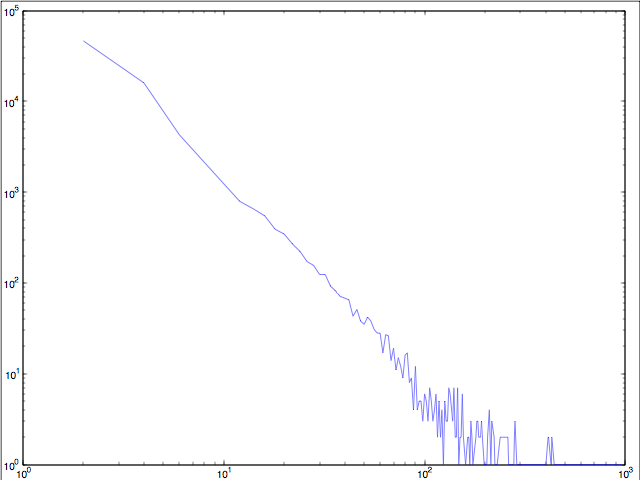
\includegraphics[width=.3\linewidth]{FIG/as-skitter.75000-indd.png}}\hfill
\subfloat[Out-Degree Distribution\label{fig:as-skitter_outdegree}]
  {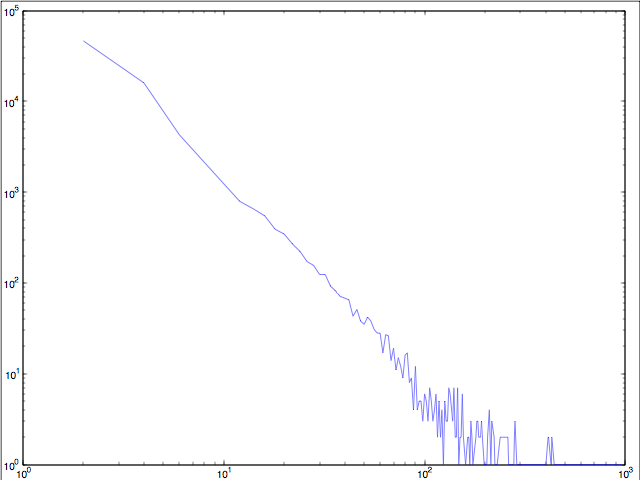
\includegraphics[width=.3\linewidth]{FIG/as-skitter.75000-outdd.png}}\hfill
\subfloat[Degree Distribution\label{fig:as-skitter_degree}]
  {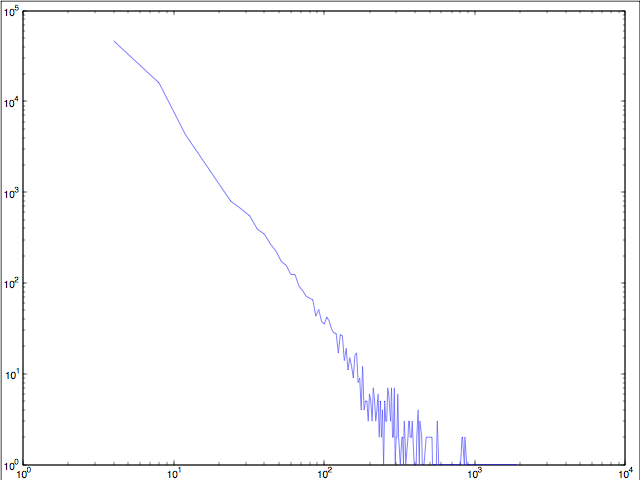
\includegraphics[width=.3\linewidth]{FIG/as-skitter.75000-dd.png}}
\caption{Degree Distributions of as-skitter\label{fig:as-skitter_degree_dist}}
\end{figure}
\begin{figure}
\subfloat[In-Degree Distribution\label{fig:ca-AstroPh_indegree}]
  {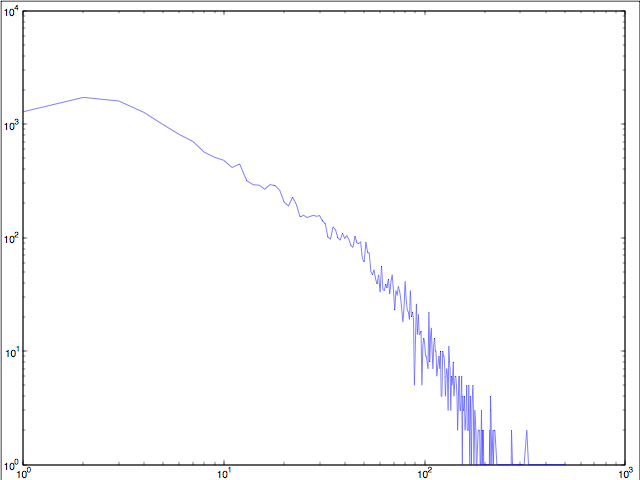
\includegraphics[width=.3\linewidth]{FIG/ca-AstroPh-indd.png}}\hfill
\subfloat[Out-Degree Distribution\label{fig:ca-AstroPh_outdegree}]
  {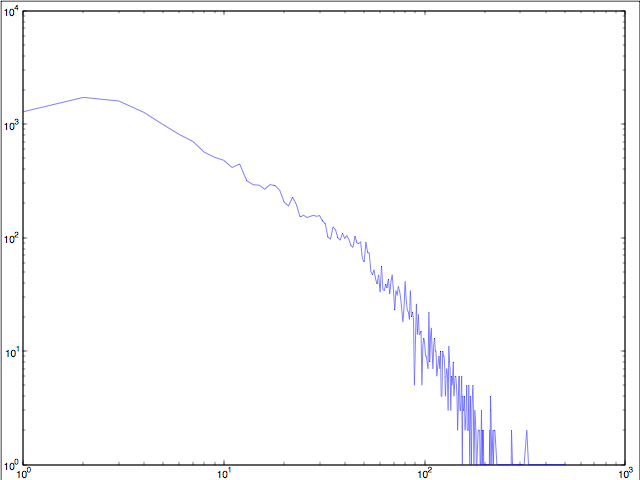
\includegraphics[width=.3\linewidth]{FIG/ca-AstroPh-outdd.png}}\hfill
\subfloat[Degree Distribution\label{fig:ca-AstroPh_degree}]
  {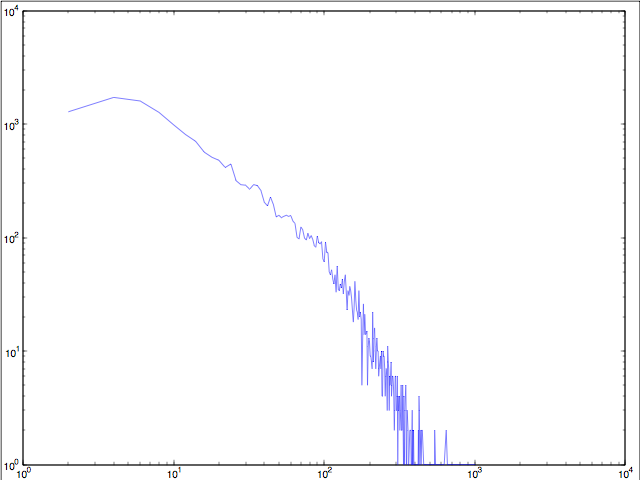
\includegraphics[width=.3\linewidth]{FIG/ca-AstroPh-dd.png}}
\caption{Degree Distributions of a-AstroPh\label{fig:ca-AstroPh_degree_dist}}
\end{figure}
\begin{figure}
\subfloat[In-Degree Distribution\label{fig:cit-HepPh_indegree}]
  {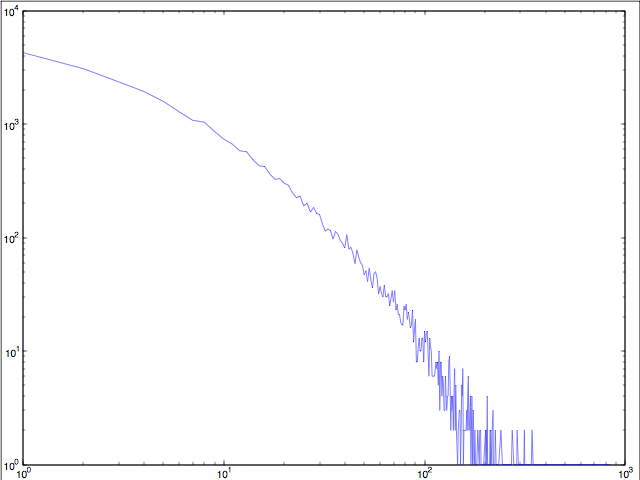
\includegraphics[width=.3\linewidth]{FIG/cit-HepPh-indd.png}}\hfill
\subfloat[Out-Degree Distribution\label{fig:cit-HepPh_outdegree}]
  {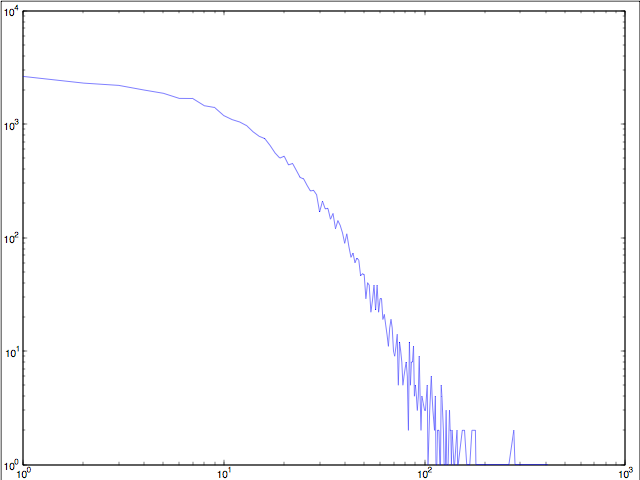
\includegraphics[width=.3\linewidth]{FIG/cit-HepPh-outdd.png}}\hfill
\subfloat[Degree Distribution\label{fig:cit-HepPh_degree}]
  {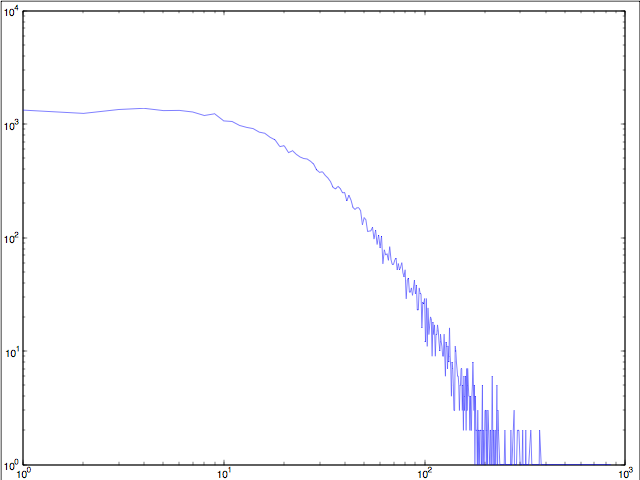
\includegraphics[width=.3\linewidth]{FIG/cit-HepPh-dd.png}}
\caption{Degree Distributions of cit-HepPh\label{fig:cit-HepPh_degree_dist}}
\end{figure}
\begin{figure}
\subfloat[In-Degree Distribution\label{fig:cit-HepTh_indegree}]
  {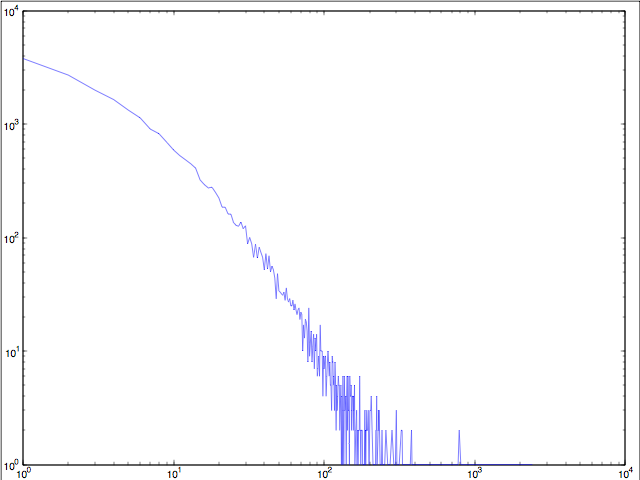
\includegraphics[width=.3\linewidth]{FIG/cit-HepTh-indd.png}}\hfill
\subfloat[Out-Degree Distribution\label{fig:cit-HepTh_outdegree}]
  {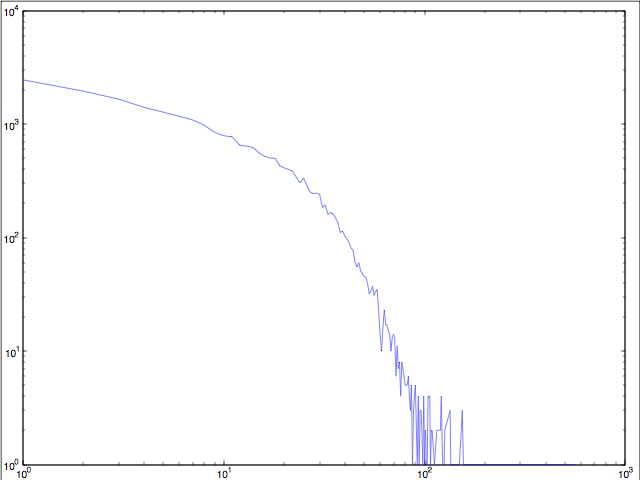
\includegraphics[width=.3\linewidth]{FIG/cit-HepTh-outdd.png}}\hfill
\subfloat[Degree Distribution\label{fig:cit-HepTh_degree}]
  {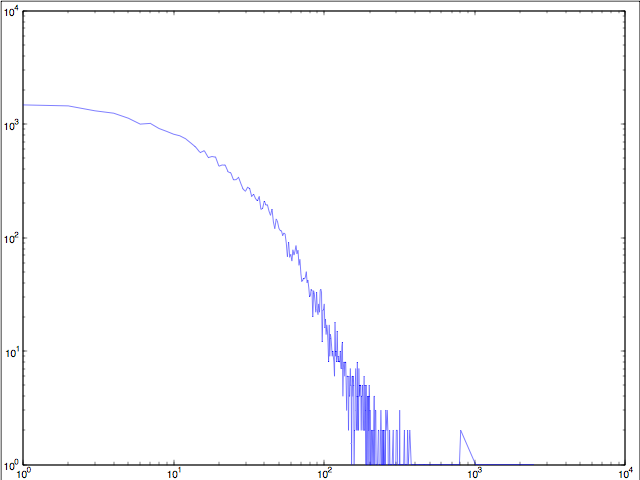
\includegraphics[width=.3\linewidth]{FIG/cit-HepTh-dd.png}}
\caption{Degree Distributions of cit-HepTh\label{fig:cit-HepTh_degree_dist}}
\end{figure}
\begin{figure}
\subfloat[In-Degree Distribution\label{fig:com-amazon.ungraph_indegree}]
  {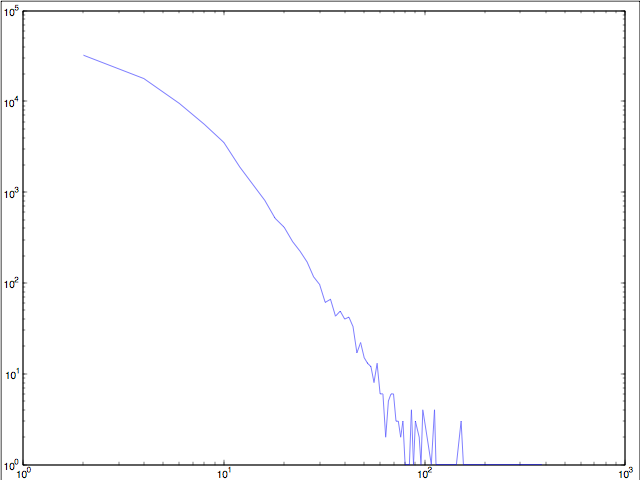
\includegraphics[width=.3\linewidth]{FIG/com-amazon.ungraph-indd.png}}\hfill
\subfloat[Out-Degree Distribution\label{fig:com-amazon.ungraph_outdegree}]
  {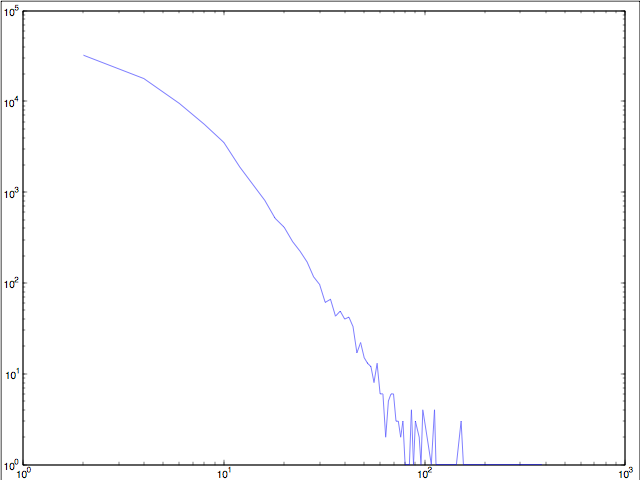
\includegraphics[width=.3\linewidth]{FIG/com-amazon.ungraph-outdd.png}}\hfill
\subfloat[Degree Distribution\label{fig:com-amazon.ungraph_degree}]
  {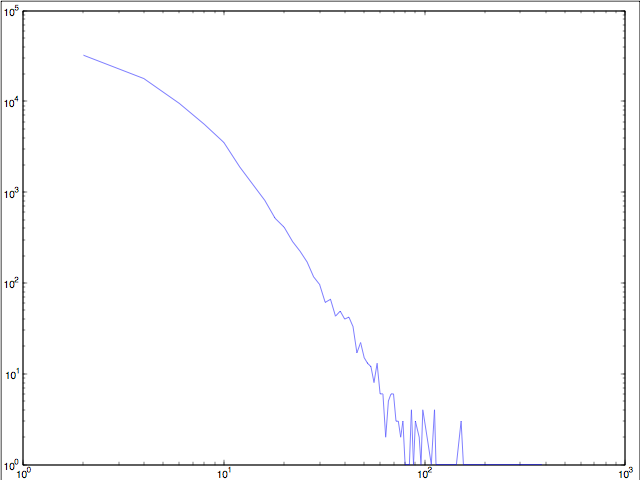
\includegraphics[width=.3\linewidth]{FIG/com-amazon.ungraph-dd.png}}
\caption{Degree Distributions of com-amazon.ungraph\label{fig:com-amazon.ungraph_degree_dist}}
\end{figure}
\begin{figure}
\subfloat[In-Degree Distribution\label{fig:com-dblp.ungraph_indegree}]
  {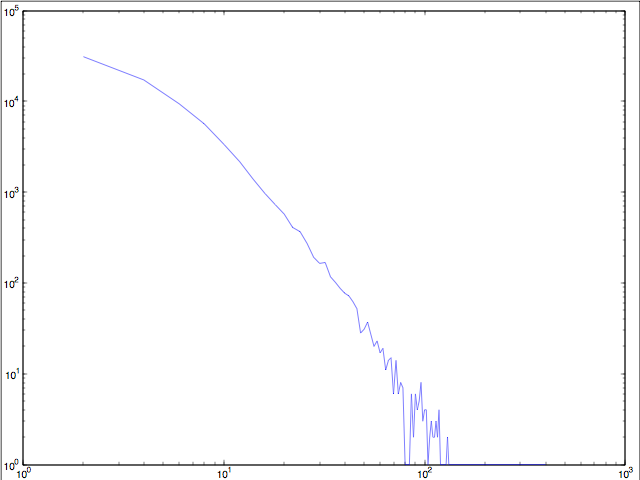
\includegraphics[width=.3\linewidth]{FIG/com-dblp.ungraph-indd.png}}\hfill
\subfloat[Out-Degree Distribution\label{fig:com-dblp.ungraph_outdegree}]
  {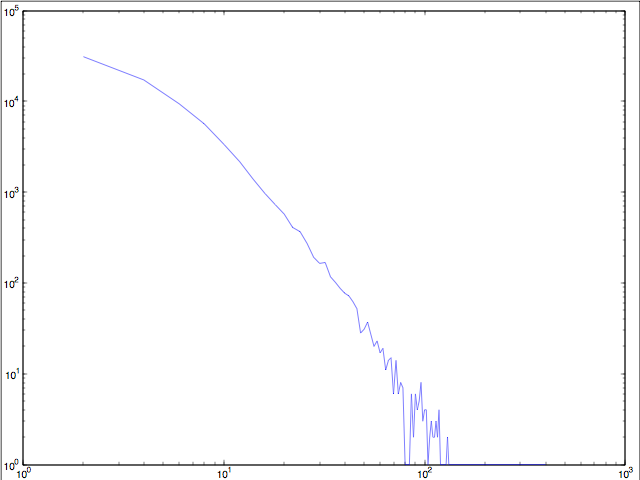
\includegraphics[width=.3\linewidth]{FIG/com-dblp.ungraph-outdd.png}}\hfill
\subfloat[Degree Distribution\label{fig:com-dblp.ungraph_degree}]
  {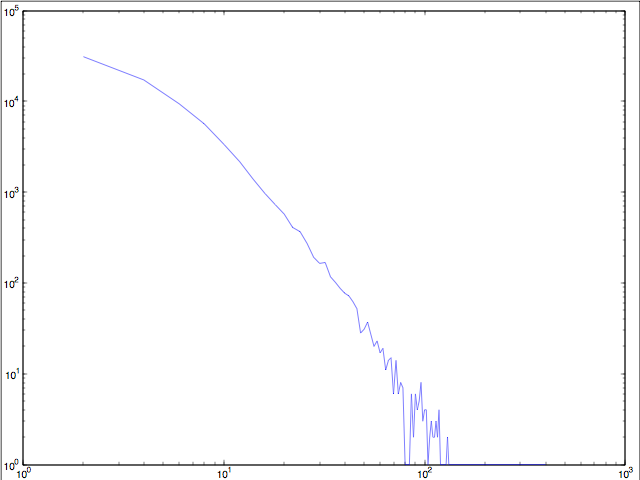
\includegraphics[width=.3\linewidth]{FIG/com-dblp.ungraph-dd.png}}
\caption{Degree Distributions of com-dblp.ungraph\label{fig:com-dblp.ungraph_degree_dist}}
\end{figure}
\begin{figure}
\subfloat[In-Degree Distribution\label{fig:email-Enron.ungraph_indegree}]
  {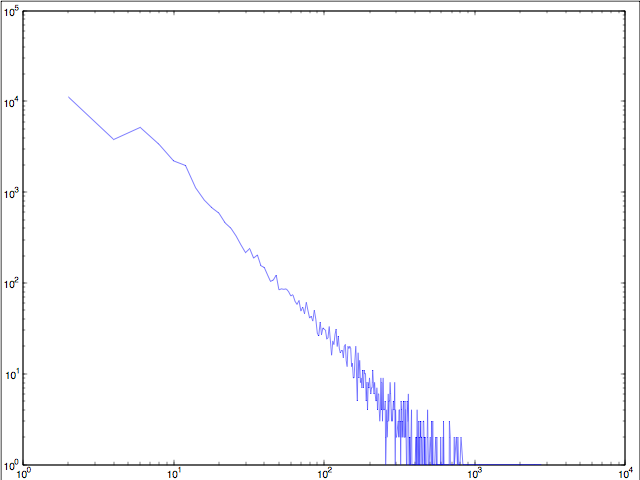
\includegraphics[width=.3\linewidth]{FIG/email-Enron.ungraph-indd.png}}\hfill
\subfloat[Out-Degree Distribution\label{fig:email-Enron.ungraph_outdegree}]
  {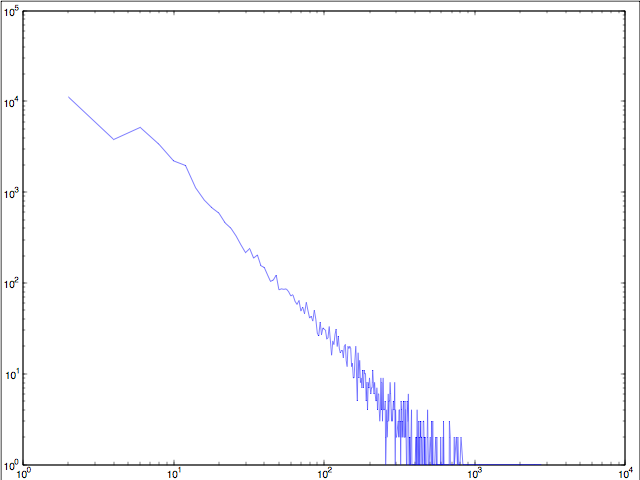
\includegraphics[width=.3\linewidth]{FIG/email-Enron.ungraph-outdd.png}}\hfill
\subfloat[Degree Distribution\label{fig:email-Enron.ungraph_degree}]
  {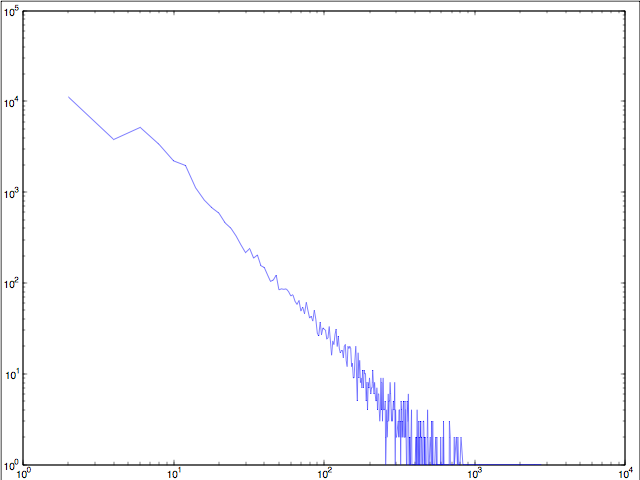
\includegraphics[width=.3\linewidth]{FIG/email-Enron.ungraph-dd.png}}
\caption{Degree Distributions of email-Enron.ungraph\label{fig:email-Enron.ungraph_degree_dist}}
\end{figure}
\begin{figure}
\subfloat[In-Degree Distribution\label{fig:email-EuAll_indegree}]
  {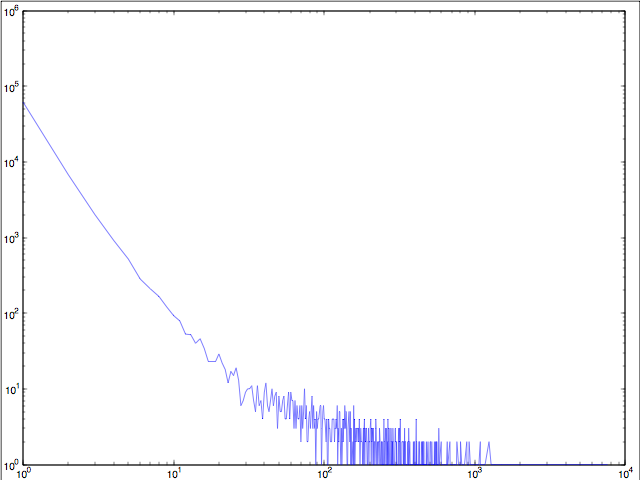
\includegraphics[width=.3\linewidth]{FIG/email-EuAll-indd.png}}\hfill
\subfloat[Out-Degree Distribution\label{fig:email-EuAll_outdegree}]
  {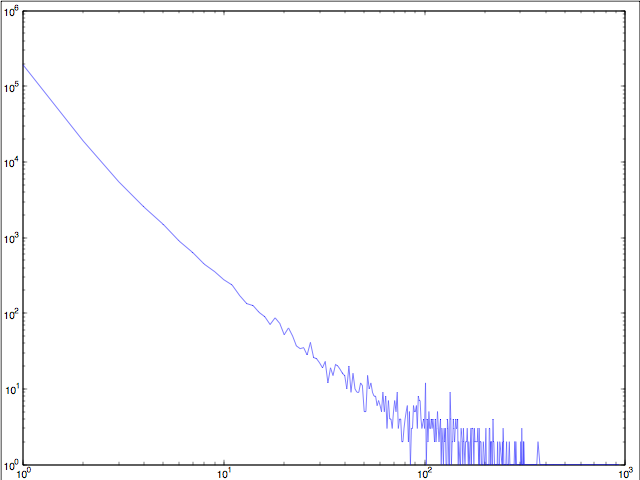
\includegraphics[width=.3\linewidth]{FIG/email-EuAll-outdd.png}}\hfill
\subfloat[Degree Distribution\label{fig:email-EuAll_degree}]
  {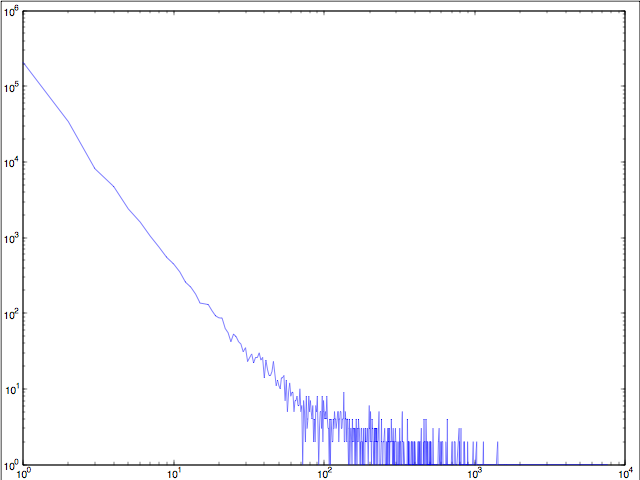
\includegraphics[width=.3\linewidth]{FIG/email-EuAll-dd.png}}
\caption{Degree Distributions of email-EuAll\label{fig:email-EuAll_degree_dist}}
\end{figure}
\begin{figure}
\subfloat[In-Degree Distribution\label{fig:p2p-Gnutella31_indegree}]
  {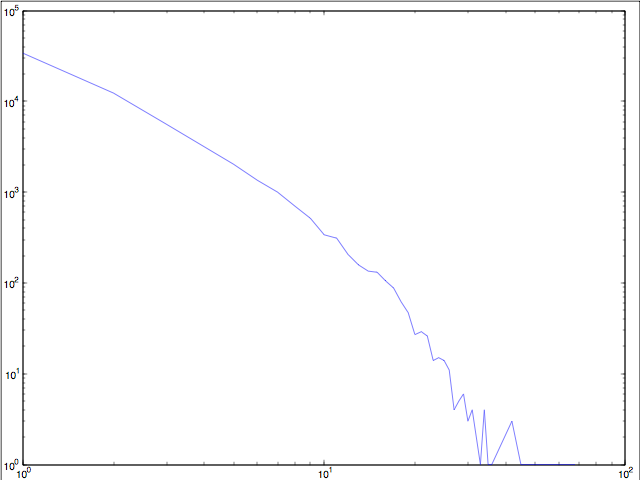
\includegraphics[width=.3\linewidth]{FIG/p2p-Gnutella31-indd.png}}\hfill
\subfloat[Out-Degree Distribution\label{fig:p2p-Gnutella31_outdegree}]
  {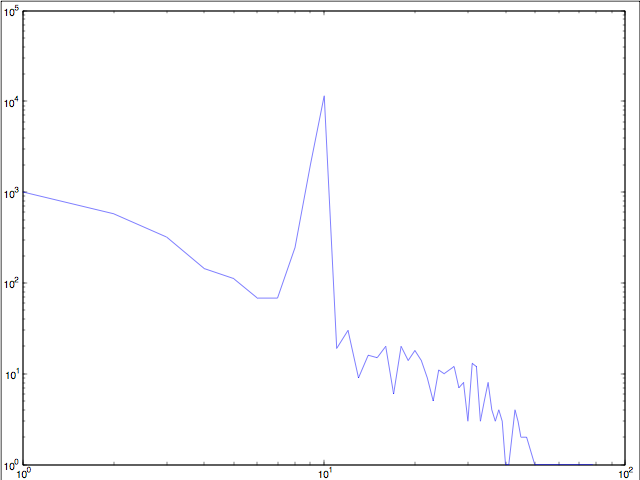
\includegraphics[width=.3\linewidth]{FIG/p2p-Gnutella31-outdd.png}}\hfill
\subfloat[Degree Distribution\label{fig:p2p-Gnutella31_degree}]
  {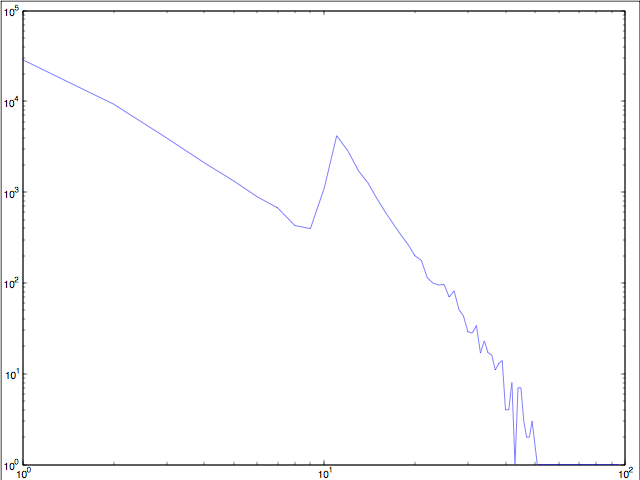
\includegraphics[width=.3\linewidth]{FIG/p2p-Gnutella31-dd.png}}
\caption{Degree Distributions of p2p-Gnutella31\label{fig:p2p-Gnutella31_degree_dist}}
\end{figure}
\begin{figure}
\label{deg_last}
\subfloat[In-Degree Distribution\label{fig:soc-Slashdot0811_indegree}]
  {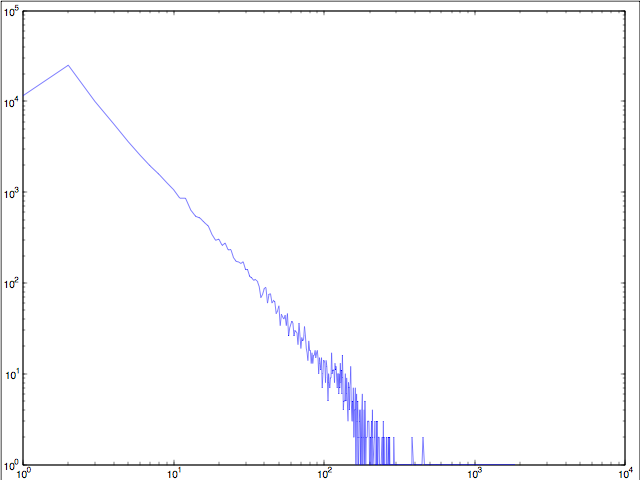
\includegraphics[width=.3\linewidth]{FIG/soc-Slashdot0811-indd.png}}\hfill
\subfloat[Out-Degree Distribution\label{fig:soc-Slashdot0811_outdegree}]
  {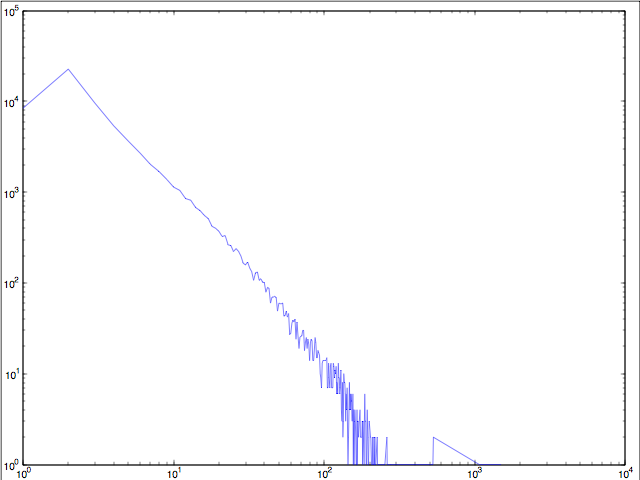
\includegraphics[width=.3\linewidth]{FIG/soc-Slashdot0811-outdd.png}}\hfill
\subfloat[Degree Distribution\label{fig:soc-Slashdot0811_degree}]
  {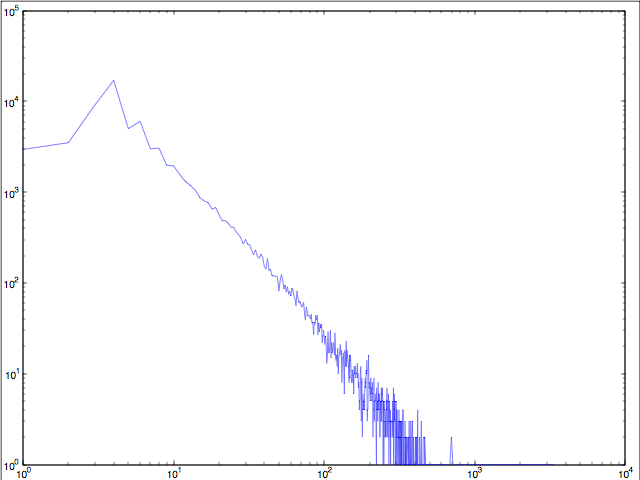
\includegraphics[width=.3\linewidth]{FIG/soc-Slashdot0811-dd.png}}
\caption{Degree Distributions of soc-Slashdot0811\label{fig:soc-Slashdot0811_degree_dist}}
\end{figure}
\begin{figure}
\subfloat[In-Degree Distribution\label{fig:as-Caida.undir_indegree}]
  {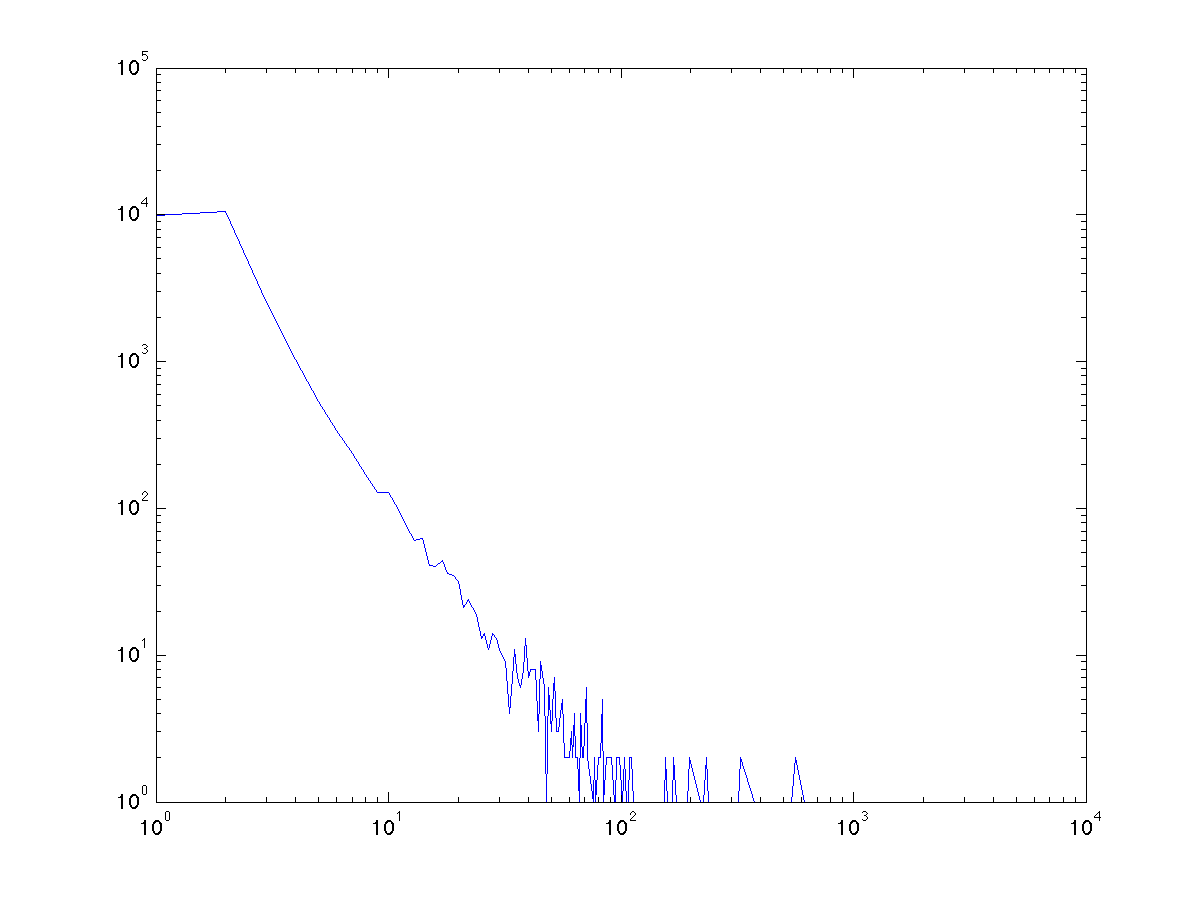
\includegraphics[width=.3\linewidth]{FIG/as-Caida.undir.txt-indegreedist.png}}\hfill
\subfloat[Out-Degree Distribution\label{fig:as-Caida.undir_outdegree}]
  {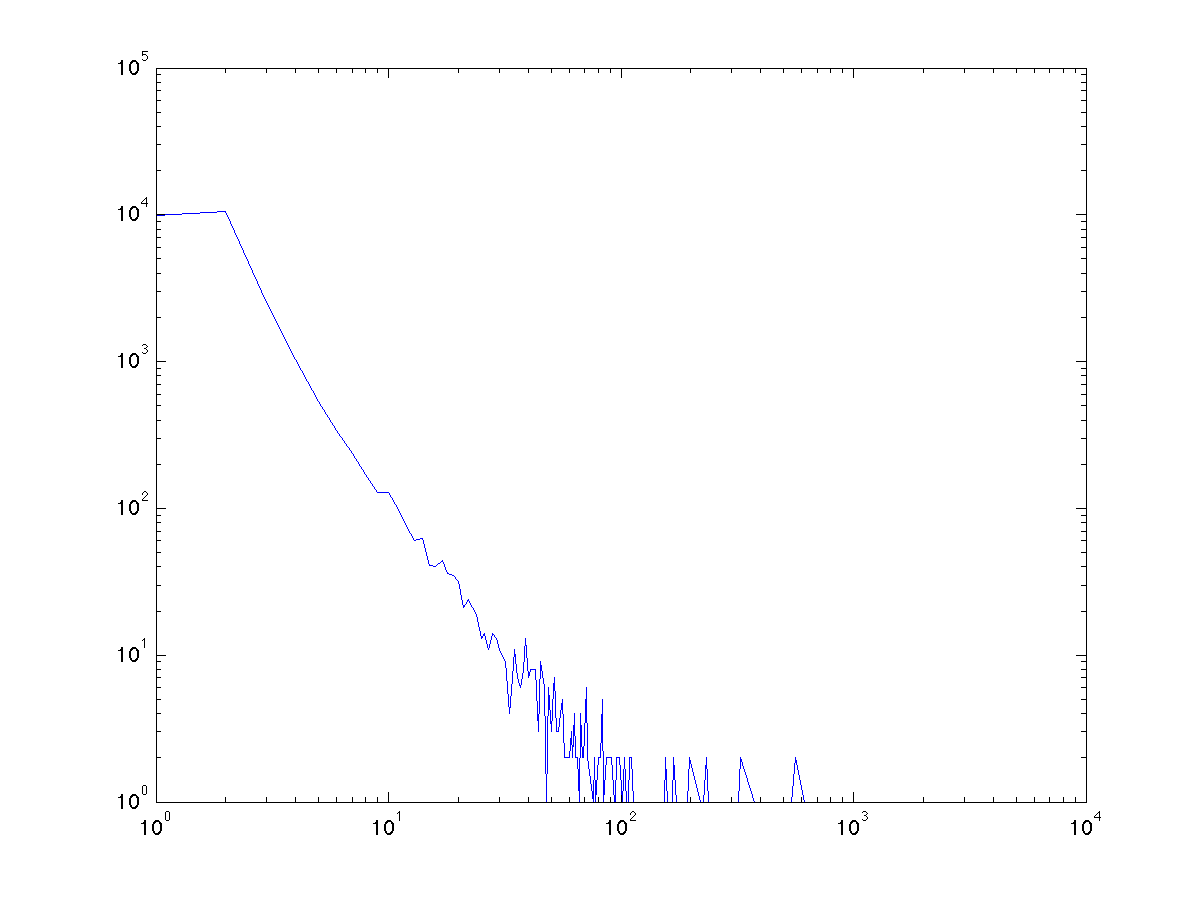
\includegraphics[width=.3\linewidth]{FIG/as-Caida.undir.txt-outdegreedist.png}}\hfill
\subfloat[Degree Distribution\label{fig:as-Caida.undir_degree}]
  {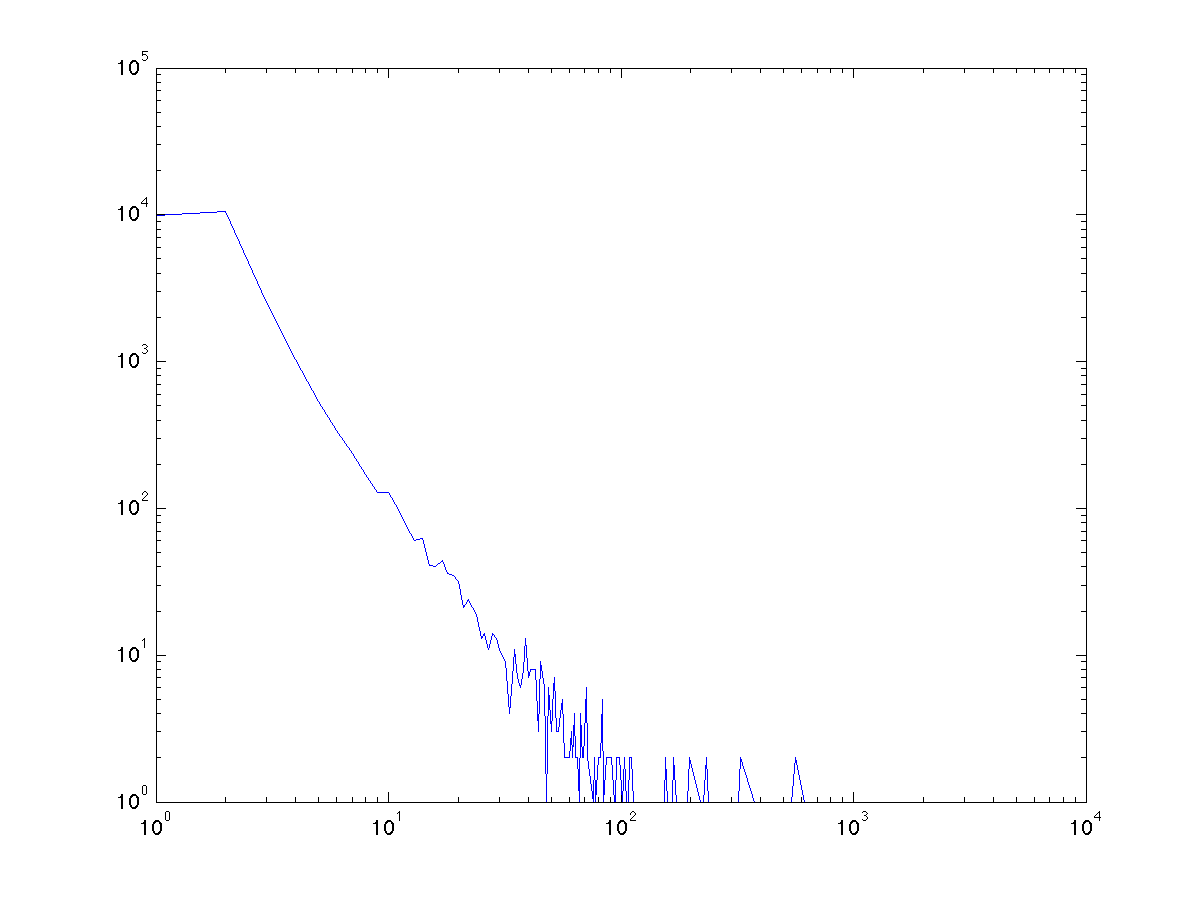
\includegraphics[width=.3\linewidth]{FIG/as-Caida.undir.txt-degree.png}}
\caption{Degree Distributions of as-Caida\label{fig:as-Caida.undir.txt_degree_dist}}
\end{figure}
\begin{figure}
\subfloat[In-Degree Distribution\label{fig:bio-protein_indegree}]
  {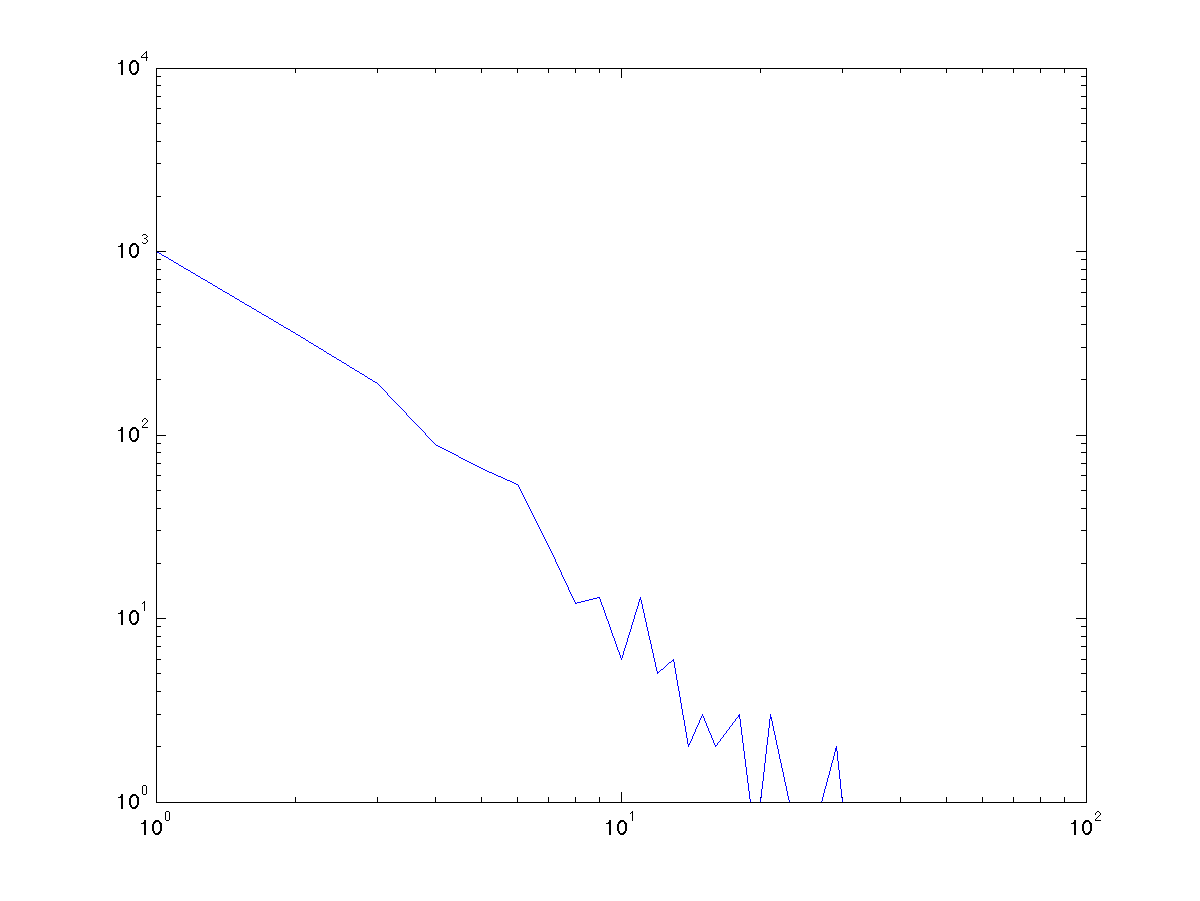
\includegraphics[width=.3\linewidth]{FIG/bio-protein-undir.txt-indegreedist.png}}\hfill
\subfloat[Out-Degree Distribution\label{fig:bio-protein_outdegree}]
  {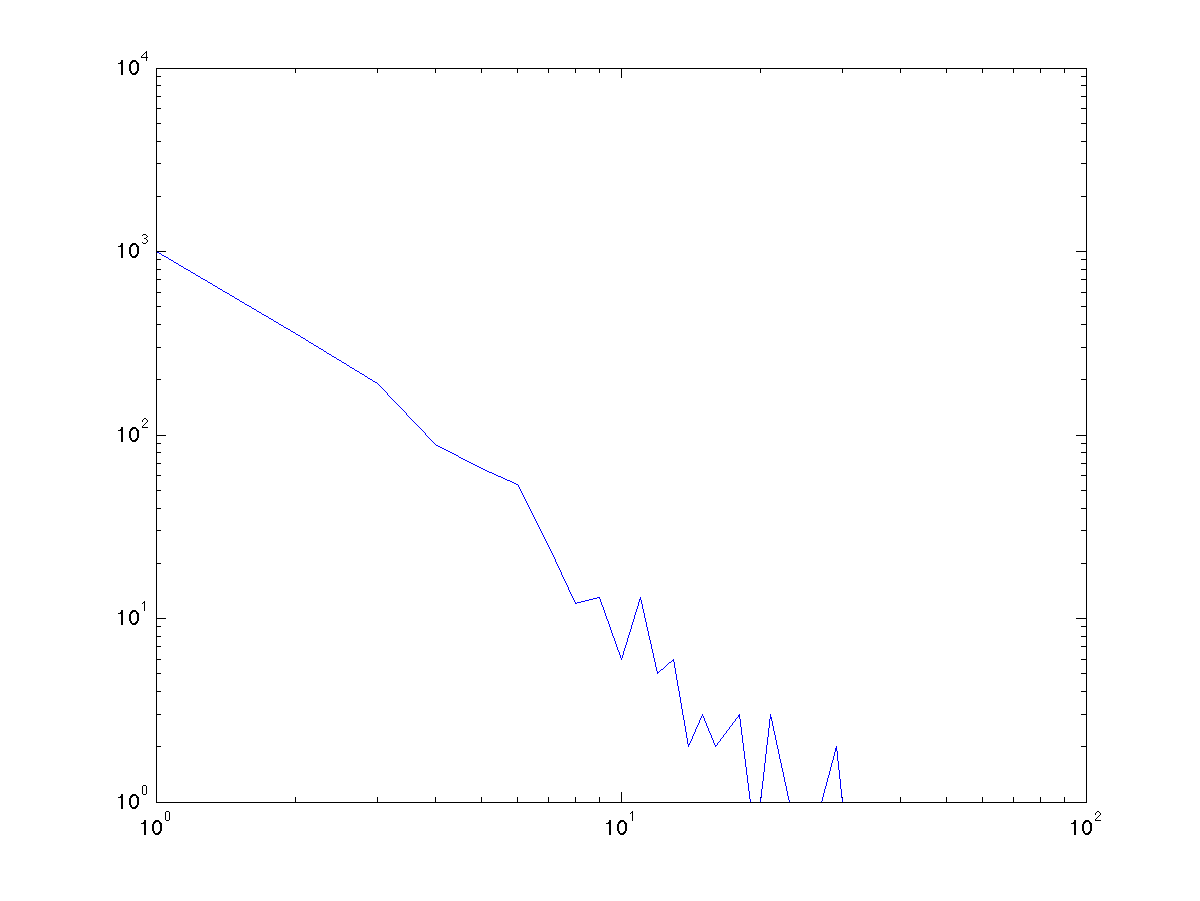
\includegraphics[width=.3\linewidth]{FIG/bio-protein-undir.txt-outdegreedist.png}}\hfill
\subfloat[Degree Distribution\label{fig:bio-protein_degree}]
  {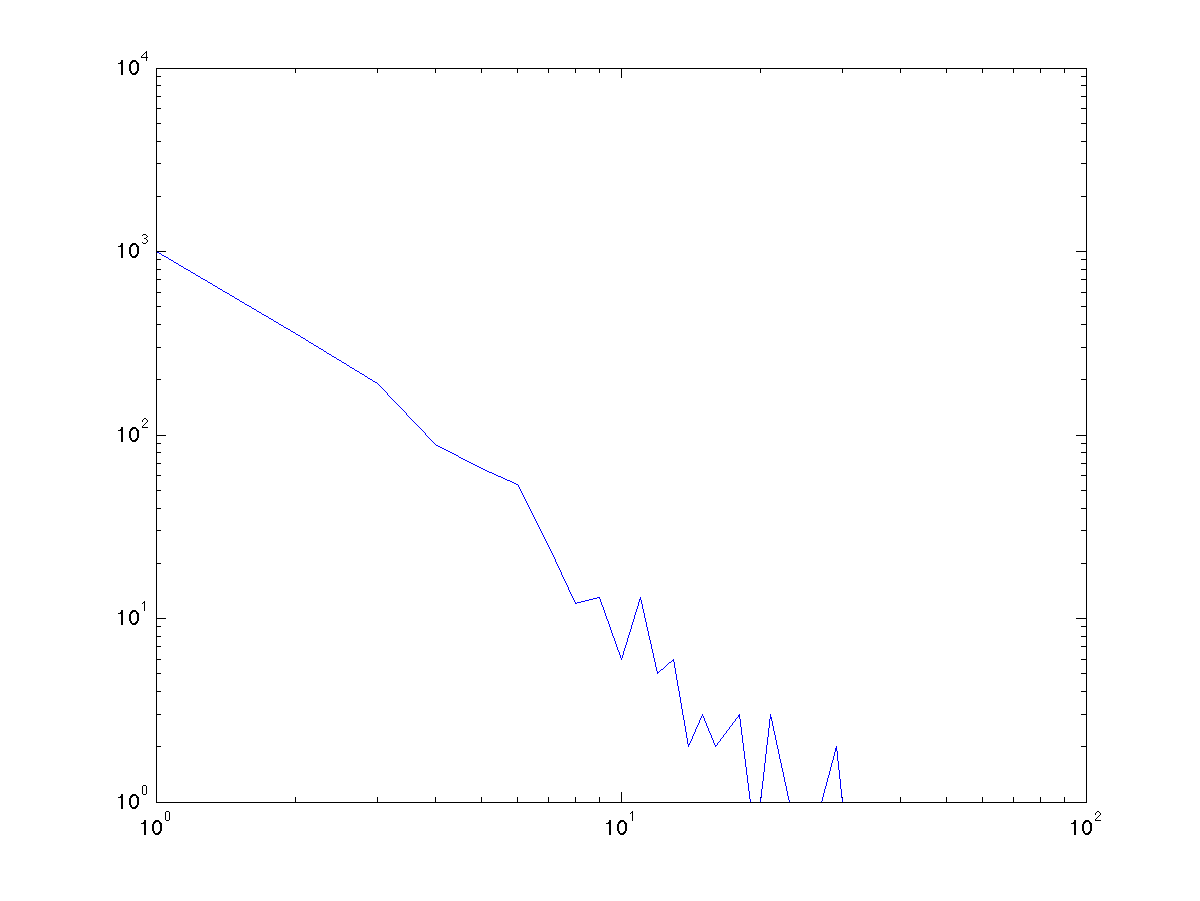
\includegraphics[width=.3\linewidth]{FIG/bio-protein-undir.txt-degree.png}}
\caption{Degree Distributions of bio-protein\label{fig:bio-protein_degree_dist}}
\end{figure}
\begin{figure}
\subfloat[In-Degree Distribution\label{fig:cit-Cora_indegree}]
  {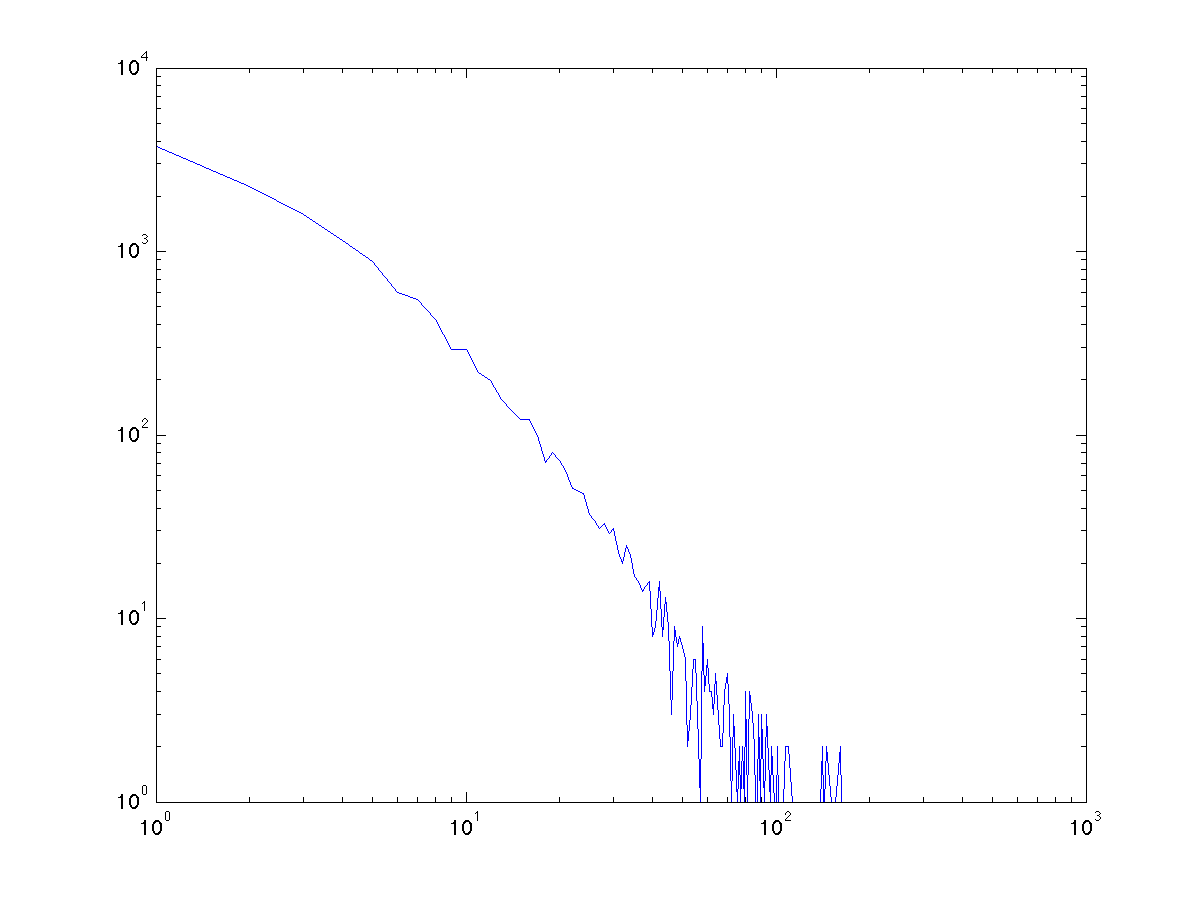
\includegraphics[width=.3\linewidth]{FIG/cit-Cora.txt-indegreedist.png}}\hfill
\subfloat[Out-Degree Distribution\label{fig:cit-Cora_outdegree}]
  {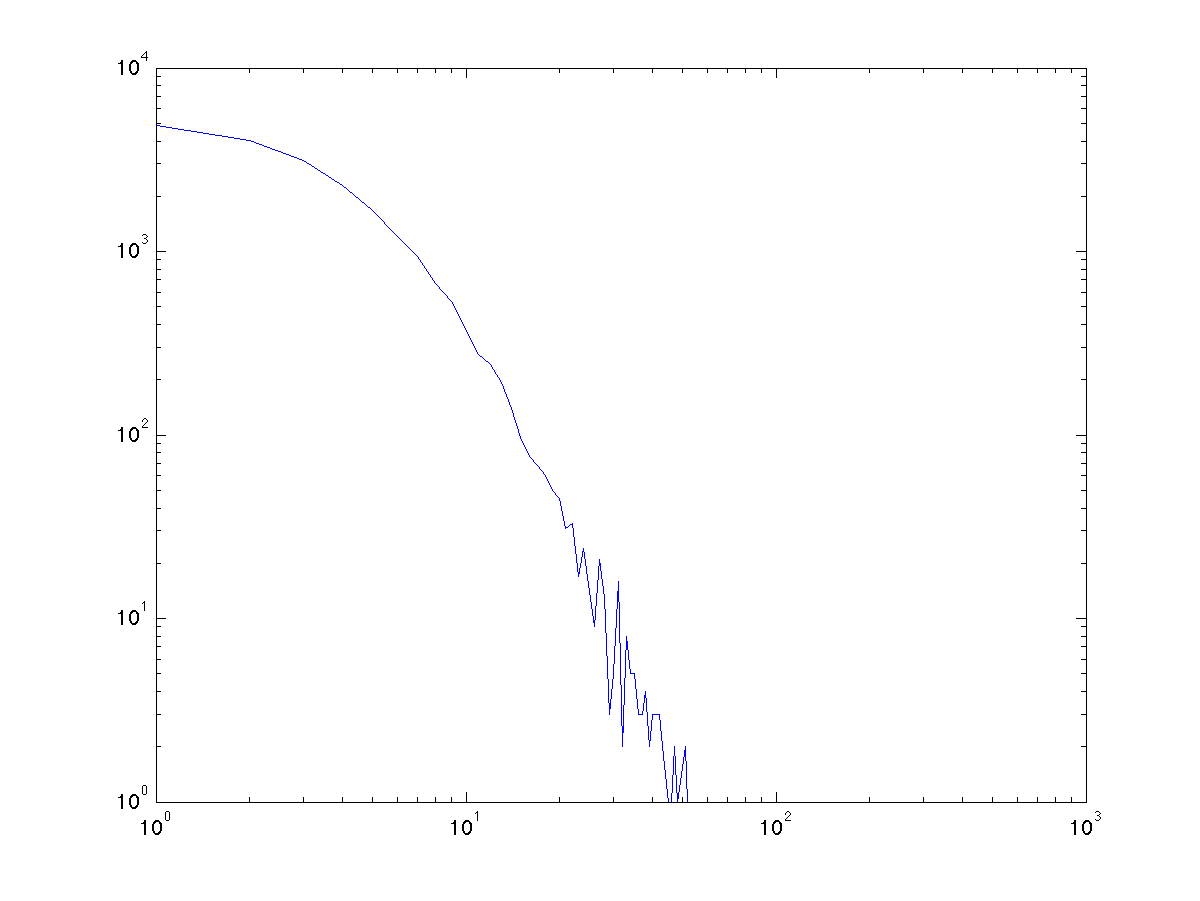
\includegraphics[width=.3\linewidth]{FIG/cit-Cora.txt-outdegreedist.png}}\hfill
\subfloat[Degree Distribution\label{fig:cit-Cora_degree}]
  {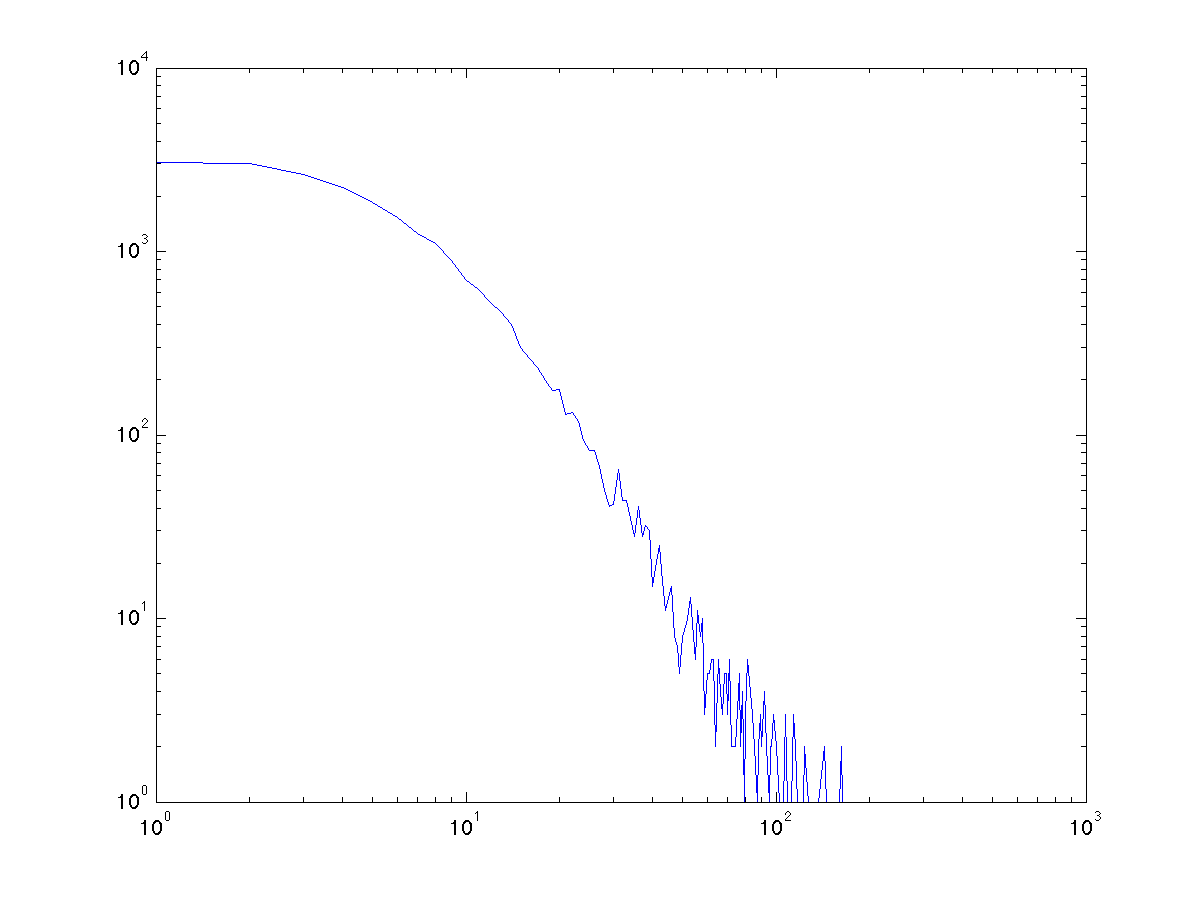
\includegraphics[width=.3\linewidth]{FIG/cit-Cora.txt-degree.png}}
\caption{Degree Distributions of cit-Cora\label{fig:cit-Cora_degree_dist}}
\end{figure}
\begin{figure}
\subfloat[In-Degree Distribution\label{fig:soc-digg_indegree}]
  {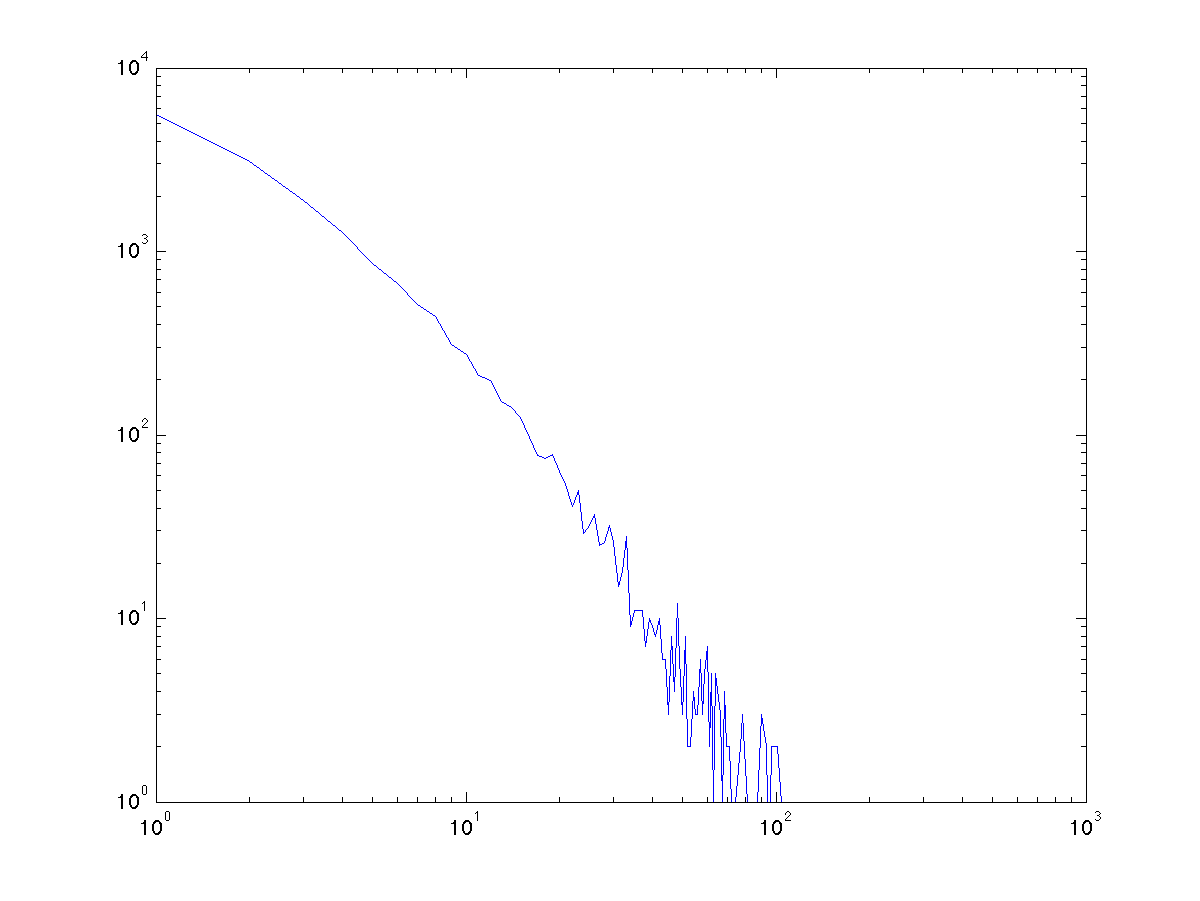
\includegraphics[width=.3\linewidth]{FIG/soc-digg.txt-indegreedist.png}}\hfill
\subfloat[Out-Degree Distribution\label{fig:soc-digg_outdegree}]
  {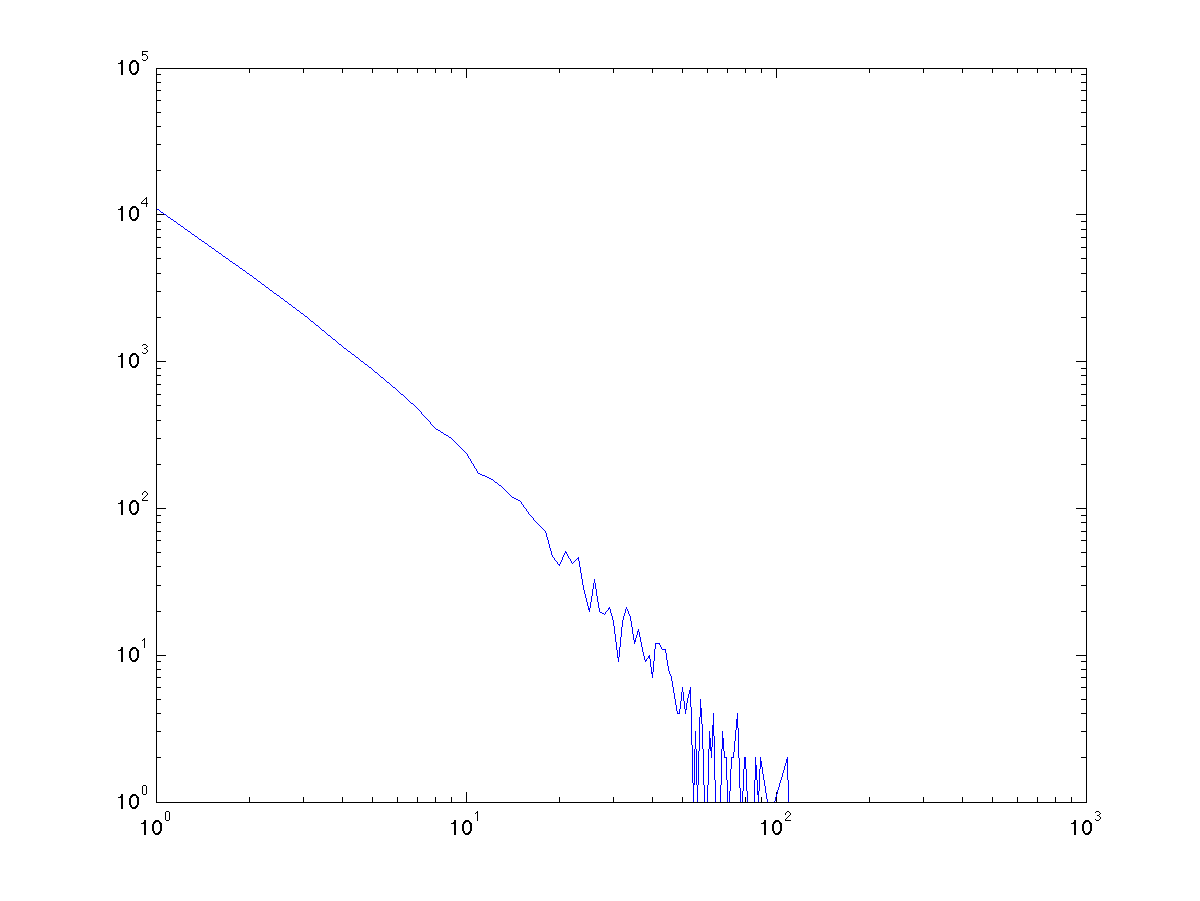
\includegraphics[width=.3\linewidth]{FIG/soc-digg.txt-outdegreedist.png}}\hfill
\subfloat[Degree Distribution\label{fig:soc-digg_degree}]
  {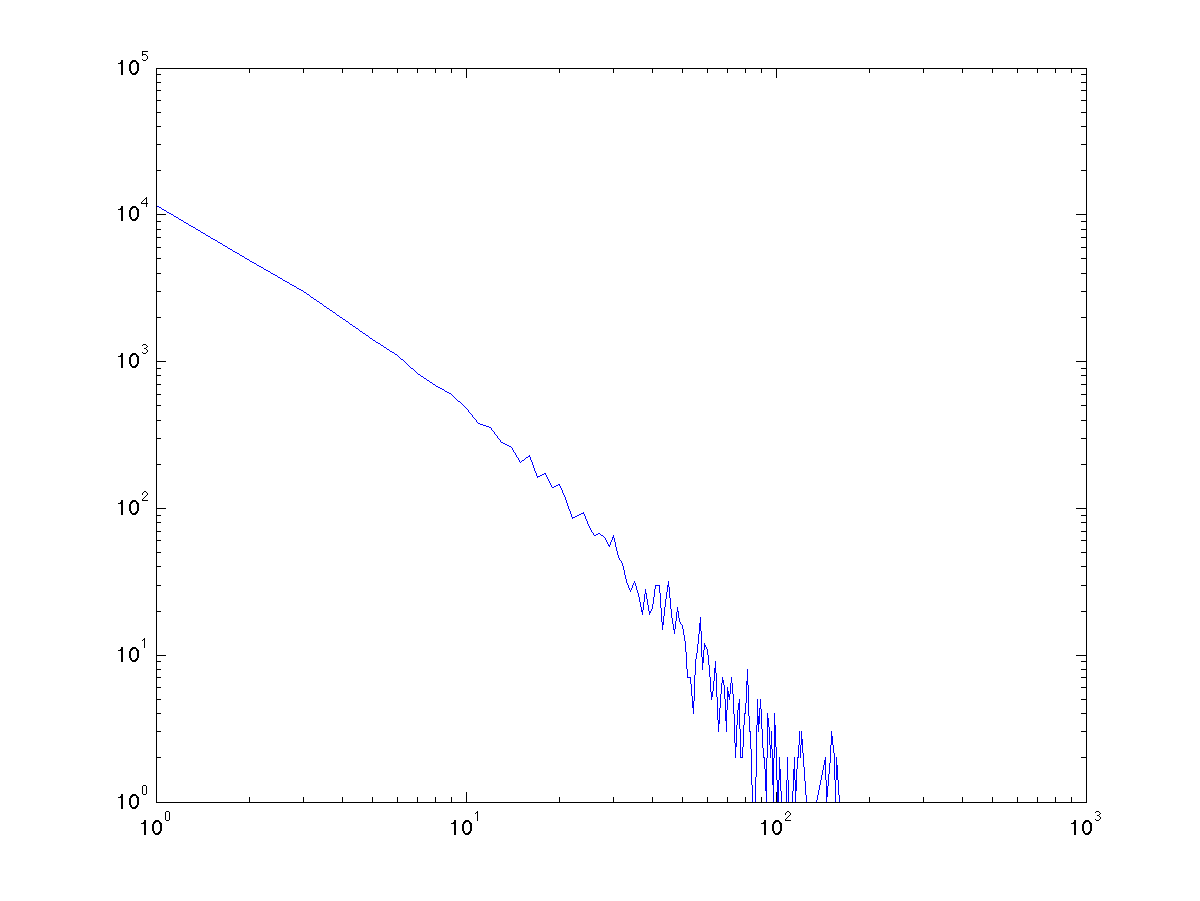
\includegraphics[width=.3\linewidth]{FIG/soc-digg.txt-degree.png}}
\caption{Degree Distributions of soc-digg\label{fig:soc-digg_degree_dist}}
\end{figure}
\begin{figure}
\subfloat[In-Degree Distribution\label{fig:soc-flickr_indegree}]
  {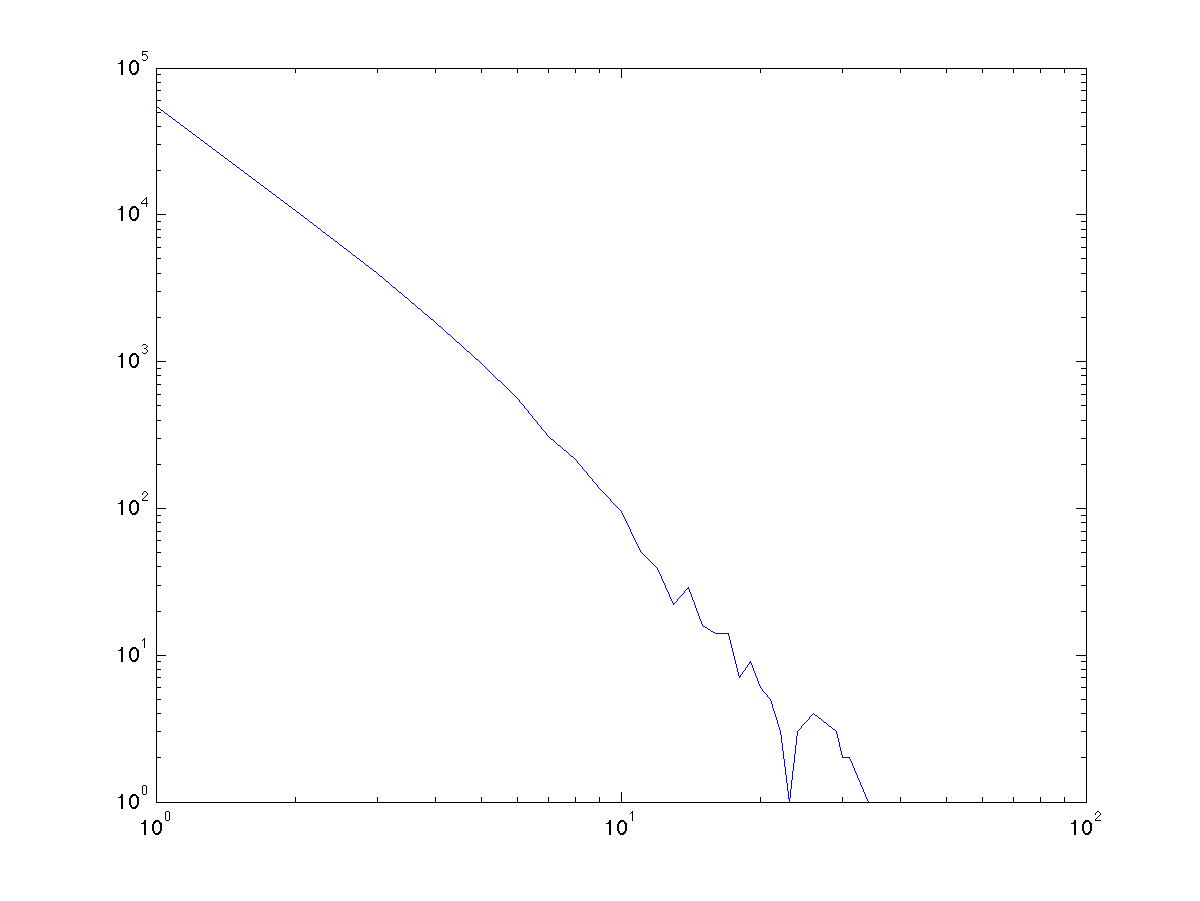
\includegraphics[width=.3\linewidth]{FIG/soc-flickr-75000.txt-indegreedist.png}}\hfill
\subfloat[Out-Degree Distribution\label{fig:soc-flickr_outdegree}]
  {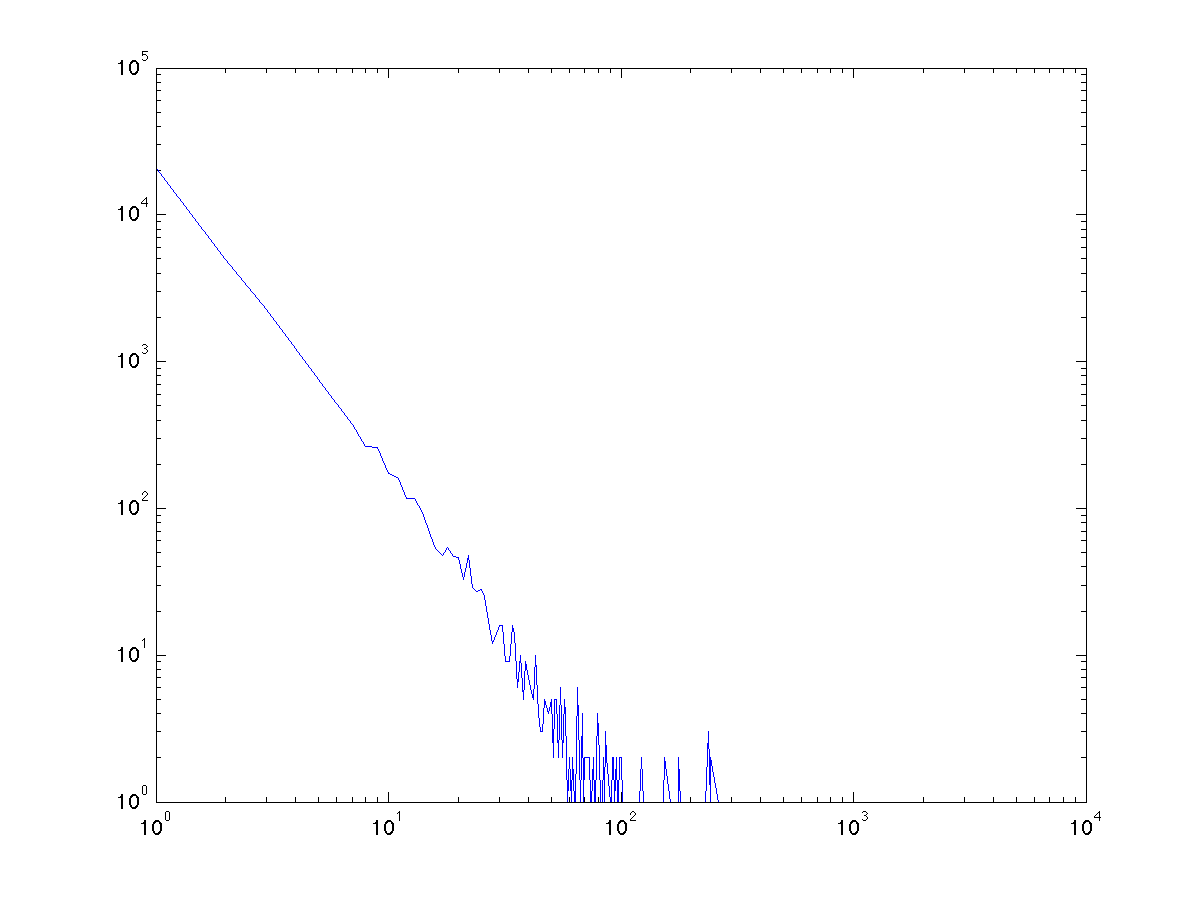
\includegraphics[width=.3\linewidth]{FIG/soc-flickr-75000.txt-outdegreedist.png}}\hfill
\subfloat[Degree Distribution\label{fig:soc-flickr_degree}]
  {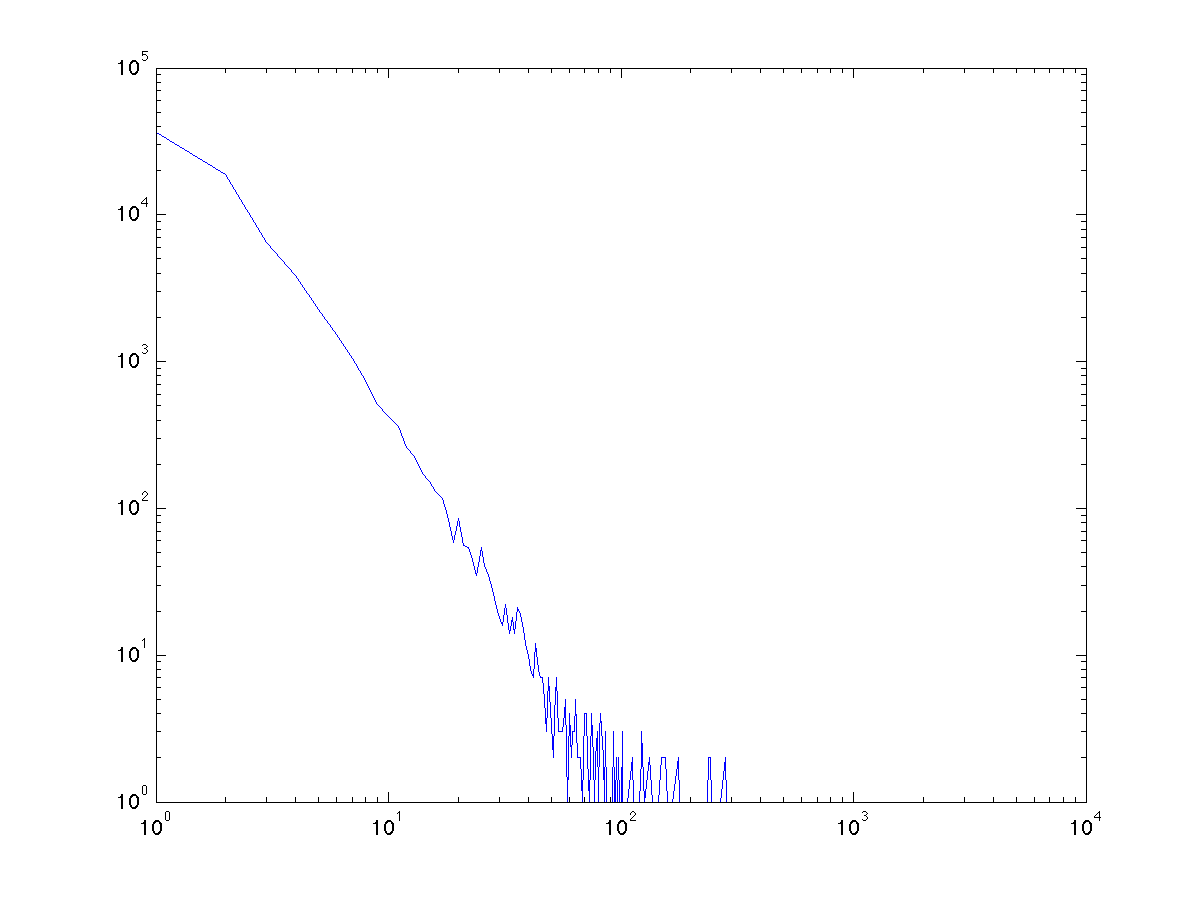
\includegraphics[width=.3\linewidth]{FIG/soc-flickr-75000.txt-degree.png}}
\caption{Degree Distributions of soc-flickr\label{fig:soc-flickr_degree_dist}}
\end{figure}
\begin{figure}
\subfloat[In-Degree Distribution\label{fig:soc-hamsterster_indegree}]
  {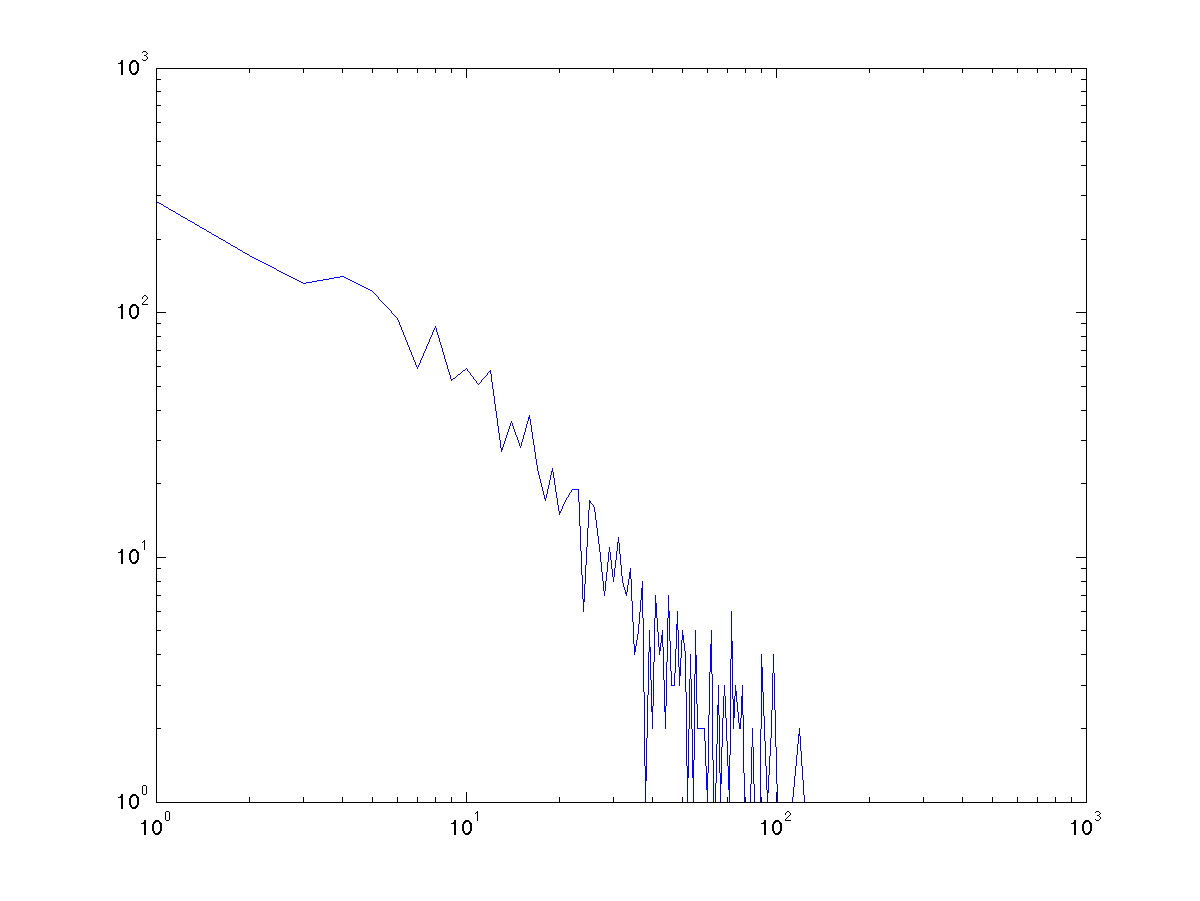
\includegraphics[width=.3\linewidth]{FIG/soc-hamsterster.undir.txt-indegreedist.png}}\hfill
\subfloat[Out-Degree Distribution\label{fig:soc-hamsterster_outdegree}]
  {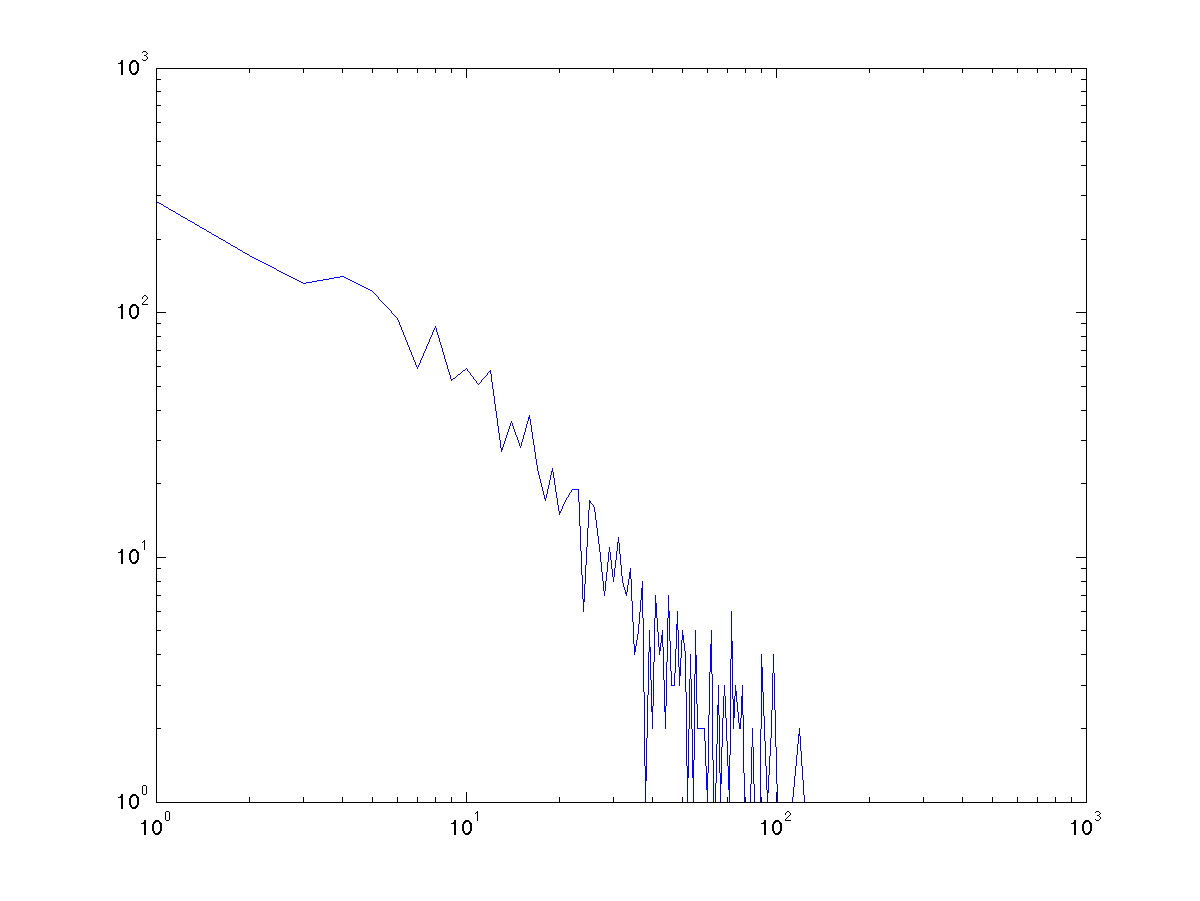
\includegraphics[width=.3\linewidth]{FIG/soc-hamsterster.undir.txt-outdegreedist.png}}\hfill
\subfloat[Degree Distribution\label{fig:soc-hamsterster_degree}]
  {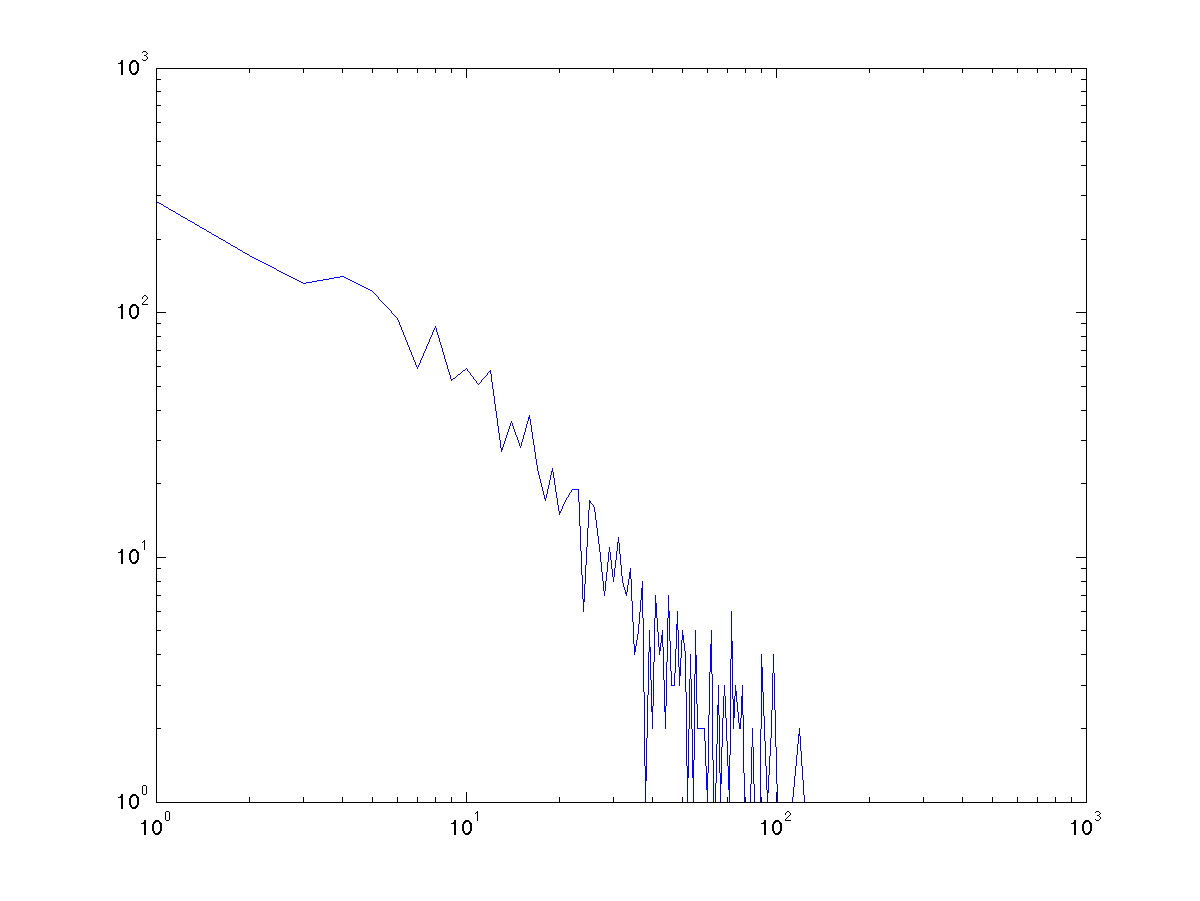
\includegraphics[width=.3\linewidth]{FIG/soc-hamsterster.undir.txt-degree.png}}
\caption{Degree Distributions of soc-hamsterster\label{fig:soc-hamsterster_degree_dist}}
\end{figure}
\begin{figure}
\subfloat[In-Degree Distribution\label{fig:soc-pokec_indegree}]
  {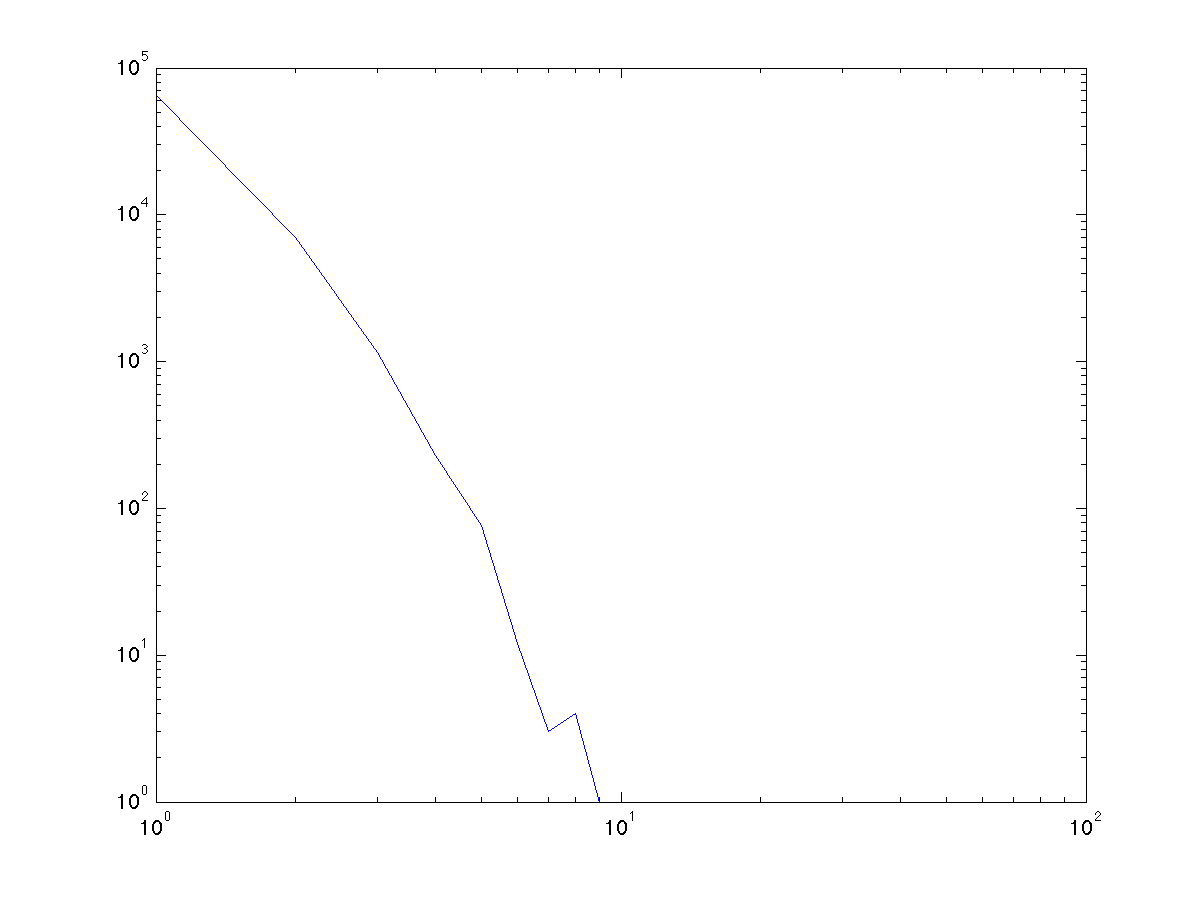
\includegraphics[width=.3\linewidth]{FIG/soc-pokec-75000.txt-indegreedist.png}}\hfill
\subfloat[Out-Degree Distribution\label{fig:soc-pokec_outdegree}]
  {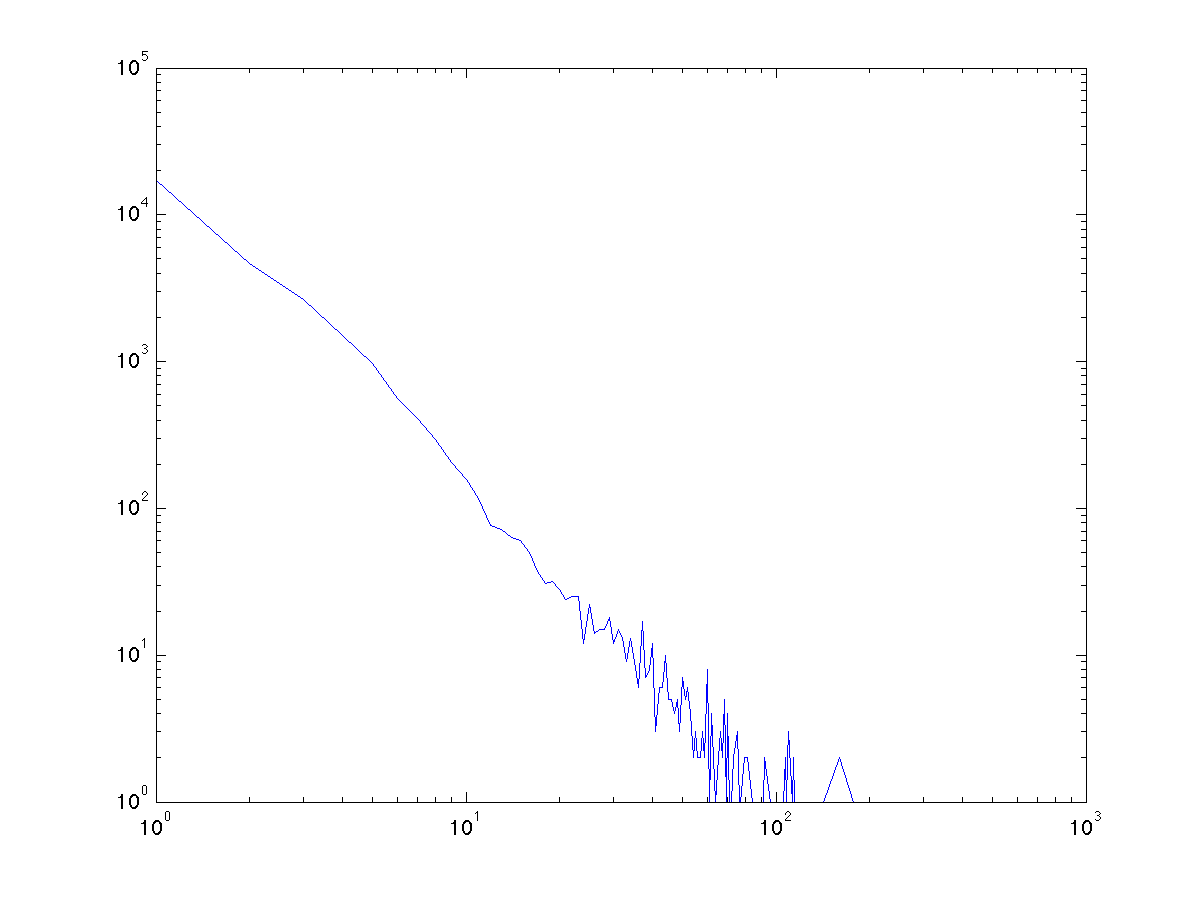
\includegraphics[width=.3\linewidth]{FIG/soc-pokec-75000.txt-outdegreedist.png}}\hfill
\subfloat[Degree Distribution\label{fig:soc-pokec_degree}]
  {\includegraphics[width=.3\linewidth]{FIG/soc-pokec-75000.txt-degree.png}}
\caption{Degree Distributions of soc-pokec\label{fig:soc-pokec_degree_dist}}
\end{figure}
\begin{figure}
\subfloat[In-Degree Distribution\label{fig:soc-Youtube_indegree}]
  {\includegraphics[width=.3\linewidth]{FIG/soc-Youtube-75000.undir.txt-indegreedist.png}}\hfill
\subfloat[Out-Degree Distribution\label{fig:soc-Youtube_outdegree}]
  {\includegraphics[width=.3\linewidth]{FIG/soc-Youtube-75000.undir.txt-outdegreedist.png}}\hfill
\subfloat[Degree Distribution\label{fig:soc-Youtube_degree}]
  {\includegraphics[width=.3\linewidth]{FIG/soc-Youtube-75000.undir.txt-degree.png}}
\caption{Degree Distributions of soc-Youtube\label{fig:soc-Youtube_degree_dist}}
\end{figure}

\clearpage

\begin{figure}
\subfloat[In-Degree Distribution\label{fig:soft-jdkdependency_indegree}]
  {\includegraphics[width=.3\linewidth]{FIG/soft-jdkdependency.txt-indegreedist.png}}\hfill
\subfloat[Out-Degree Distribution\label{fig:soft-jdkdependency_outdegree}]
  {\includegraphics[width=.3\linewidth]{FIG/soft-jdkdependency.txt-outdegreedist.png}}\hfill
\subfloat[Degree Distribution\label{fig:soft-jdkdependency_degree}]
  {\includegraphics[width=.3\linewidth]{FIG/soft-jdkdependency.txt-degree.png}}
\caption{Degree Distributions of soft-jdkdependency\label{fig:soft-jdkdependency_degree_dist}}
\end{figure}
\begin{figure}
\subfloat[In-Degree Distribution\label{fig:text-spanishbook_indegree}]
  {\includegraphics[width=.3\linewidth]{FIG/text-spanishbook.txt-indegreedist.png}}\hfill
\subfloat[Out-Degree Distribution\label{fig:text-spanishbook_outdegree}]
  {\includegraphics[width=.3\linewidth]{FIG/text-spanishbook.txt-outdegreedist.png}}\hfill
\subfloat[Degree Distribution\label{figt:ext-spanishbook_degree}]
  {\includegraphics[width=.3\linewidth]{FIG/text-spanishbook.txt-degree.png}}
\caption{Degree Distributions of text-spanishbook\label{fig:text-spanishbook_degree_dist}}
\end{figure}



\subsubsection{Weakly Connected Component and Triangle count}
\textbf{Global Pattern} \\
We find that most graphs consist of a small number of groups (compared with the total number of nodes). And most nodes are in one biggest groups. \\
And the triangle number illustrates how nodes in groups are connected to each other. \\
\\
\textbf{Strange Behaviors} \\
\begin{itemize} 
\item p2p-Gnutella31 has 12 components. This shows the nodes in this graph are highly connected. But the triangle count is little. So it seems that there are several popular nodes in this graph. And most nodes connect to these popular servers instead of connecting to each others. \\
\item cit-HepPh has 61 components and the triangle count is a large number. This shows the nodes in this graph are mostly connected to each others. \\
\item email-EuAll has 15836 components. Although the maximun component size is huge, the connections between nodes are not strong. It illustrates people are more likely to form small discussion groups in daily work communication.\\
\item ca-AstroPh and email-Enron have extremely high triangle counts. Which shows the nodes in these 2 graphs are very densely connected.\\
\item Nodes in as-Caida are all connected. And the triangles is much more than nodes number. Which indicates the graph is very dense. \\
\item Nodes in cit-Cora are also all connected. But the triangle number is not large compared with the nodes number. So this graph is more likely to be a star type graph (highly centralize).\\
\item In soc-hamsterster, triangles number is huge compared with members in each components. This shows that each components are highly connected. So the members in each components are very related with each other.\\
\item soc-pokec has extremely small triangles number(4.8). Which indicates the graph is highly centralize in each sub groups.\\
\item soft-jdkdependency and text-spanishbook both have large triangles numbers and all connected. The graphs are very dense. \\
\end{itemize} 
\scalebox{0.8}{
\begin{tabular}{| l | c | c | c | c | c |} \hline
\textbf{Metrics} & \textbf{as-skitter} & \textbf{ca-AstroPh} & \textbf{cit-HepPh} & \textbf{cit-HepTh} & \textbf{com-amazon} \\ \hline
components & 310 & 290 & 61 & 143 & 1946 \\ \hline
max group & 69768 & 17926 & 34454 & 27465 & 47556 \\ \hline
triangle & 28389.34144 & 1061822.808 & 60696.51906 & 191035.2798 & 132.7590596 \\ \hline
\end{tabular}}\\
\\
\\
\scalebox{0.8}{
\begin{tabular}{| l | c | c | c | c | c |} \hline
\textbf{Metrics} & \textbf{com-dblp} & \textbf{email-Enron} & \textbf{email-EuAll} & \textbf{p2p-Gnutella31} & \textbf{soc-Slashdot0811} \\ \hline
components & 949 & 1065 & 15836 & 12 & 2091\\ \hline
max group & 67361 & 33696 & 224832 & 62561 & 72780\\ \hline
triangle & 786.338039 & 2059367.367 & 370075.0779 & 307.5803753 & 252186.8962\\ \hline
\end{tabular}}\\
\\
\\
\scalebox{0.8}{
\begin{tabular}{| l | c | c | c | c | c |} \hline
\textbf{Metrics} & \textbf{as-Caida} & \textbf{bio-protein} & \textbf{cit-Cora} & \textbf{soc-digg} & \textbf{soc-flickr} \\ \hline
components & 1 & 173 & 1 & 373 & 1280 \\ \hline
max group & 26475 & 1458 & 23166 & 29652 & 63529 \\ \hline
triangle & 29967.0841542 & 30.1742701786 & 3192.44451312 & 5207.40905806 & 1574.17467495 \\ \hline
\end{tabular}}\\
\\
\\
\scalebox{0.8}{
\begin{tabular}{| l | c | c | c | c | c |} \hline
\textbf{Metrics} & \textbf{soc-hamsterster} & \textbf{soc-pokec} & \textbf{soc-Youtube} & \textbf{soft-jdkdependency} & \textbf{text-spanishbook} \\ \hline
components & 23 & 113 & 4319 & 1 & 1\\ \hline
max group & 1788 & 73564 & 54143 & 6434 & 12643\\ \hline
triangle & 15328.5846289 & 4.77180117934 & 100.71969417 & 150378.549887 & 191251.983102\\ \hline
\end{tabular}}\\

\subsubsection{PageRank}

\begin{figure}
\subfloat[as-skitter.75000\label{fig:as-skitter}]
  {\includegraphics[width=.25\linewidth]{FIG/pagerank/as-skitter_75000.png}}\hfill
\subfloat[ca-AstroPh\label{fig:ca-AstroPh}]
  {\includegraphics[width=.25\linewidth]{FIG/pagerank/ca-AstroPh.png}}\hfill
\subfloat[cit-HepPh\label{fig:cit-HepPh}]
  {\includegraphics[width=.25\linewidth]{FIG/pagerank/cit-HepPh.png}} \hfill
\subfloat[cit-HepTh\label{fig:cit-HepTh}]
  {\includegraphics[width=.25\linewidth]{FIG/pagerank/cit-HepTh.png}}\hfill
\subfloat[com-amazon.ungraph-75000\label{fig:com-amazon.ungraph-75000}]
  {\includegraphics[width=.25\linewidth]{FIG/pagerank/com-amazon.ungraph-75000.png}}\hfill
\subfloat[com-dblp.ungraph-75000\label{fig:com-dblp.ungraph-75000}]
  {\includegraphics[width=.25\linewidth]{FIG/pagerank/com-dblp.ungraph-75000.png}} \hfill
 \subfloat[email-Enron.ungraph\label{fig:email-Enron.ungraph}]
  {\includegraphics[width=.25\linewidth]{FIG/pagerank/email-Enron.ungraph.png}}\hfill
\subfloat[email-EuAll\label{fig:email-EuAll}]
  {\includegraphics[width=.25\linewidth]{FIG/pagerank/email-EuAll.png}}\hfill
\subfloat[p2p-Gnutella31\label{fig:p2p-Gnutella31}]
  {\includegraphics[width=.25\linewidth]{FIG/pagerank/p2p-Gnutella31.png}} \hfill
 \subfloat[soc-Slashdot0811-75000\label{fig:soc-Slashdot0811-75000}]
  {\includegraphics[width=.25\linewidth]{FIG/pagerank/soc-Slashdot0811-75000.png}} 
 \subfloat[as-Caida\label{fig:as-Caida}]
  {\includegraphics[width=.25\linewidth]{FIG/pagerank/as-Caida.undir.txt.png}} \hfill  
 \subfloat[bio-protein\label{fig:bio-protein}]
  {\includegraphics[width=.25\linewidth]{FIG/pagerank/bio-protein-undir.txt.png}} \hfill  
 \subfloat[cit-Cora\label{fig:cit-Cora}]
  {\includegraphics[width=.25\linewidth]{FIG/pagerank/cit-Cora.txt.png}} \hfill 
 \subfloat[soc-digg\label{fig:soc-digg}]
  {\includegraphics[width=.25\linewidth]{FIG/pagerank/soc-digg.txt.png}} \hfill  
 \subfloat[soc-flickr-75000\label{fig:soc-flickr-75000}]
  {\includegraphics[width=.25\linewidth]{FIG/pagerank/soc-flickr-75000.txt.png}} \hfill  
 \subfloat[soc-hamsterster\label{fig:soc-hamsterster}]
  {\includegraphics[width=.25\linewidth]{FIG/pagerank/soc-hamsterster.undir.txt.png}} \hfill  
 \subfloat[soc-pokec-75000\label{fig:soc-pokec-75000}]
  {\includegraphics[width=.25\linewidth]{FIG/pagerank/soc-pokec-75000.txt.png}} \hfill  
 \subfloat[soc-Youtube-75000\label{fig:soc-Youtube-75000}]
  {\includegraphics[width=.25\linewidth]{FIG/pagerank/soc-Youtube-75000.undir.txt.png}} \hfill  
 \subfloat[soft-jdkdependency\label{fig:soft-jdkdependency}]
  {\includegraphics[width=.25\linewidth]{FIG/pagerank/soft-jdkdependency.txt.png}} \hfill  
 \subfloat[text-spanishbook\label{fig:text-spanishbook}]
  {\includegraphics[width=.25\linewidth]{FIG/pagerank/text-spanishbook.txt.png}} \hfill  
\caption{Pagerank value Distributions of 20 graphs}
\label{fig:pagerank}
\end{figure}

To analyze the patterns of PageRank in 20 graphs, we calculated the PageRank value of nodes in each graphs, aggregated the values into distribution, and plotted the distribution in log-log scale. Mainly, we wanted to check whether the distribution of PageRank values follow power law or not. At the same time, we observed the charts of distribution to find out strange patterns of PageRank.
\\
\\
\textbf{Global Pattern}
\\
\\
The experiment result (Figure. \ref{fig:pagerank}) shows that the PageRank value distribution in most of graphs follow power law.
\\
\\
\textbf{Strange Behaviors}
\\
\\
(1) Plateau in the Beginning
\\
\\
The distribution of PageRank in most of graphs follow power low; however, we found that there are plateaus in the beginning part of some distribution charts. Taking com-amazon.ungraph-75000 for example, the line between $10^{-8}$ and $10^{-5}$ is relative smooth. 
\\
ca-AstroPh, com-amazon.ungraph-75000, com-dblp.ungraph-75000, email-Enron.ungraph, soc-Slashdot0811-75000, as-Caida, soc-flickr-75000, soc-pokec-75000, soc-Youtube-75000, and text-spanishbook have such plateau pattern.
\\
\\
(2) Broom Tail
\\
\\
Ideally, the chart of distribution following power law would be a smooth descending straight line in log-log scale plot; however, we found that some lines of real data are not as smooth as ideal straight lines. Instead, the lines of some real data jump up and down in the last part. The shape is like a bloom.
\\
as-skitter, cit-HepTh, email-Enron.ungraph, email-EuAll, as-Caida, cit-Cora, soc-Youtube-75000, soft-jdkdependency, and text-spanishbook have such broom tail pattern.
\\
\\
(3) Vibrating Line
\\
\\
The lines in PageRank distribution chart are usually smooth, but there are some lines vibrating severely. Taking soc-hamsterster for example, its line jumps up and down severely, although the trend of line follow power-law. bio-protein and soc-hamsterster have such pattern.



\subsubsection{Eigenvalue computation (via Lanczos-SO and QR algorithms)}

\begin{center}
\scalebox{0.6}{
  \begin{tabular}{ |l | c | c | c | c | c | c |  }
    \hline
      & \textbf{cit-HepPh} & \textbf{com-amazon.ungraph-75000}  & \textbf{com-dblp.ungraph-75000}  & \textbf{email-Enron.ungraph}  & \textbf{soc-Slashdot0811-75000}  \\ \hline
First Eigenvalue & 71.24869215  & 12.46375985 & 18.08047143  & 232.0718265 & 124.3376448  \\ \hline
Second Eigenvalue & 15.78100055 & -10.49450063 & -9.989018866 & -52.74314639 & -74.23852603  \\ \hline
Third Eigenvalue & -11.28234916 & 2.528983265  & 3.950839681 & 16.07981363 & 3.277331459  \\ \hline
  \end{tabular}}
\end{center}

\begin{center}
\scalebox{0.6}{
  \begin{tabular}{ |l | c | c | c | c | c | c |  }
    \hline
      & \textbf{p2p-Gnutella31} & \textbf{ca-AstroPh} & \textbf{email-EuAll} & \textbf{cit-HepTh} & \textbf{as-skitter.75000}\\ \hline
First Eigenvalue & 12.26069439 & 182.7509283 & 134.5445114 & 108.0148181 & 182.7509283 \\ \hline
Second Eigenvalue & 2.714800955 & 64.42806942 & -59.94291686 & -48.59746457 & 64.42806942 \\ \hline
Third Eigenvalue & -2.60170164 & -0.449525922 & 6.537952019 & 9.103275079 & -0.449525922 \\ \hline
  \end{tabular}}
\end{center}

\begin{center}
\scalebox{0.6}{
  \begin{tabular}{ |l | c | c | c | c | c | c |  }
    \hline
      & \textbf{as-Caida.undir} & \textbf{bio-protein-undir} & \textbf{cit-Cora} & \textbf{soc-digg} & \textbf{soc-flickr-75000}\\ \hline
First Eigenvalue & 68.3693197062366 & 6.59050522092269 & 27.0826721488691 & 31.4948560594139 & 46.128302835195 \\ \hline
Second Eigenvalue & -51.89780364579 & -4.73938936859157 & -9.39990749609768 & 3.5437520638839 & -44.5991249417485 \\ \hline
Third Eigenvalue & 0.336124325308012 & 1.07545809389524 & 4.9442935842295 & -3.43736182466055 & 1.53574108698456 \\ \hline
  \end{tabular}}
\end{center}

\begin{center}
\scalebox{0.6}{
  \begin{tabular}{ |l | c | c | c | c | c | c |  }
    \hline
      & \textbf{soc-hamsterster.undir} & \textbf{soc-pokec-75000} & \textbf{soc-Youtube-75000.undir} & \textbf{soft-jdkdependency} & \textbf{text-spanishbook}\\ \hline
First Eigenvalue & 45.2761211252026 & 9.38962714926706 & 15.7609882639711 & 143.265820052228 & 124.70922072648 \\ \hline
Second Eigenvalue & -10.0662421612482 & -9.28310856022425 & -14.9067351906316 & -126.79096036676 & -92.5441274101652 \\ \hline
Third Eigenvalue & 5.6332490229777 & 0.918759752366816 & 1.16658315444281 & 2.26001659190722 & 8.30033058289115 \\ \hline
  \end{tabular}}
\end{center}



\subsubsection{K-core algorithm}
To analyze K-core value, we set k = 5, applied K-core algorithm on 20 graphs, and counted the distribution of k-core size. We were curious about the patterns of the K-core size distribution. 
\\
\\
\textbf{Global Pattern}
\\
\\
According to the result, we found that the graphs can be grouped into two types of graphs: Type I graphs and Type II graphs.
\\
\\
\textbf{Type I Graphs}
\\
\\
Type I graphs, like soc-Slashdot0811-75000, p2p-Gnutella31, email-EuAll, email-Enron.ungraph, cit-HepTh, cit-HepPh, ca-AstroPh , as-Caida, cit-Cora, soc-digg, soc-flickr-75000, soc-hamsterster, soft-jdkdependency, and ca-AstroPh, have a giant 5-core with more than 1000 nodes, which means that type I graph is densely connected. 
\\
\\
\textbf{Type II Graphs}
\\
\\
Type II graphs, like as-skitter.75000, com-dblp.ungraph-75000, com-amazon.ungraph-75000, bio-protein, soc-pokec, and soc-Youtube-75000, do not have such a giant k-core. Instead, there are many small (size $<$ 500) 5-cores in type II graphs. Moreover, some graphs even do not have 5-cores, like bio-protein, soc-pokec, and soc-Youtube-75000. It indicates that Type II graphs are not densely connected.
\\
\begin{center}
\scalebox{0.6}{
  \begin{tabular}{ |c | c | c | c | c | c | c | c | c | c | c | c | c | c |  }
    \hline
         \multicolumn{2}{|c|}{soc-Slashdot0811-75000} & \multicolumn{2}{c|}{p2p-Gnutella31} & \multicolumn{2}{c|}{email-EuAll} & \multicolumn{2}{c|}{email-Enron.ungraph} & \multicolumn{2}{c|}{cit-HepTh} & \multicolumn{2}{c|}{cit-HepPh} & \multicolumn{2}{c|}{ca-AstroPh} \\ \hline
		size & frequency & size & frequency & size & frequency & size & frequency & size & frequency & size & frequency & size & frequency  \\ \hline
		26137  & 1 &16174  & 1 & 7030 & 1 & 6 & 6 & 21181 & 1 & 28593 & 1 & 6 & 2 \\ \hline
		& & & & & & 7 & 2 & & & & & 7 & 2 \\ \hline
		& & & & & & 8 & 3 & & & & & 8 & 1 \\ \hline
		& & & & & & 9 & 1 & & & & & 11 & 1 \\ \hline
		& & & & & & 12 & 1 & & & &  & 18 & 1 \\ \hline
		& & & & & & 15 & 1 & & & &  & 12236 & 1 \\ \hline
		& & & & & & 11538 & 1 & & & & &   &  \\ \hline
  \end{tabular}}
\scalebox{0.6}{
  \begin{tabular}{ |c | c | c | c | c | c | c | c | c | c | c | c | c | c |  }
    \hline
         \multicolumn{2}{|c|}{as-Caida} & \multicolumn{2}{c|}{cit-Cora} & \multicolumn{2}{c|}{soc-digg} & \multicolumn{2}{c|}{soc-flickr-75000} & \multicolumn{2}{c|}{soc-hamsterster} & \multicolumn{2}{c|}{soft-jdkdependency} & \multicolumn{2}{c|}{ca-AstroPh} \\ \hline
		size & frequency & size & frequency & size & frequency & size & frequency & size & frequency & size & frequency & size & frequency  \\ \hline
		1192  & 1 & 9355 & 1 & 6794 & 1 & 1122 & 1 & 1070 & 1 & 4869 & 1 & 3144 & 1 \\ \hline
		& & & & & & & & & & & & & \\ \hline
  \end{tabular}}  
  \\5-core distribution in Type I graphs
\end{center}

\begin{center}
\scalebox{0.6}{
  \begin{tabular}{ |c | c | c | c | c | c | c | c | c | c | c | c |  }
    \hline
         \multicolumn{2}{|c|}{as-skitter.75000} & \multicolumn{2}{c|}{com-dblp.ungraph-75000} & \multicolumn{2}{c|}{com-amazon.ungraph-75000} & \multicolumn{2}{c|}{bio-protein}  & \multicolumn{2}{c|}{soc-pokec}  & \multicolumn{2}{c|}{soc-Youtube-75000}  \\ \hline
		size & frequency & size & frequency & size & frequency & size & frequency & size & frequency & size & frequency   \\ \hline
		14  & 1 & 6 & 9 & 6 & 1 & 6 & 1 & 0 & 0 & 0 & 0 \\ \hline
		181 & 1 & 7 & 3 & & & & & & & &  \\ \hline
		& & 8 & 3 & & & & & & & & \\ \hline
		& & 9 & 1 & & & & & & & & \\ \hline
		& & 10 & 1 & & & & & & & & \\ \hline
		& & 13 & 1 & & & & & & & & \\ \hline
		& & 15 & 1 & & & & & & & & \\ \hline
  \end{tabular}}
    \\5-core distribution in Type II graphs
\end{center}


	
\section{Division of Labour}
	\label{sec:dl}
    \begin{itemize*}
\item
Jiajung Wang: 

\begin{itemize*}
\item
Degree Distribution optimization and experiment
\item
Weakly Connected Component optimization and experiment
\item
Triangle count optimization and experiment
\item
Organize latex files
\end{itemize*}

\item
San-Chuan Hung: 

\begin{itemize*}
\item 
PageRank optimization and experiment
\item 
K-core optimization and experiment
\item
Eigenvalue computation optimization and experiment
\item
Organize latex files
\end{itemize*}
\end{itemize*}

	
\bibliography{BIB/sanchuah}
\bibliographystyle{plain}

\end{document}
